
\section*{Общая характеристика работы}

\newcommand{\actuality}{\underline{\textbf{\actualityTXT}}}
\newcommand{\progress}{\underline{\textbf{\progressTXT}}}
\newcommand{\aim}{\underline{{\textbf\aimTXT}}}
\newcommand{\tasks}{\underline{\textbf{\tasksTXT}}}
\newcommand{\novelty}{\underline{\textbf{\noveltyTXT}}}
\newcommand{\influence}{\underline{\textbf{\influenceTXT}}}
\newcommand{\methods}{\underline{\textbf{\methodsTXT}}}
\newcommand{\defpositions}{\underline{\textbf{\defpositionsTXT}}}
\newcommand{\reliability}{\underline{\textbf{\reliabilityTXT}}}
\newcommand{\probation}{\underline{\textbf{\probationTXT}}}
\newcommand{\contribution}{\underline{\textbf{\contributionTXT}}}
\newcommand{\publications}{\underline{\textbf{\publicationsTXT}}}

{\actuality} 
Макроскопические сверхпроводящие квантовые цепи (СКЦ) --- одна из наиболее активно развивающихся областей современной экспериментальной квантовой физики. Временем её непосредственного зарождения можно считать  1999"--~2001 гг., когда в нескольких пионерских работах \cite{nakamura1999coherent,mooij1999josephson,makhlin1999josephson,orlando1999superconducting} была показана  возможность создания макроскопических когерентных квантовых объектов на основе сверхпроводников и возможность приготовления и контроля квантовых состояний таких систем. Интерес к таким системам вырос чрезвычайно быстро: ученые поняли, что на основе СКЦ принципиально возможно построить устройства, выполняющие квантовые операции, а значит, создать квантовый процессор. За 15 с небольшим лет мировым физическим сообществом проделана огромная как теоретическая, так и экспериментальная работа для реализации квантовых вычислений и демонстрации квантовых алгоритмов при помощи устройств на базе СКЦ. Поэтому в дальнейшем будем употреблять для таких схем термин <<кубит>>, подразумевая квантовую цепь, хотя и не обязательно обладающую лишь двумя квантовыми уровнями (там, где это может привести к путанице, будут даваться соотвествующие разъяснения).  Кратко перечислим полученные мировым научным сообществом результаты:
\begin{enumerate}
	\item Разработан универсальный формализм \cite{devoret1995quantum} квантования произвольного кубита, позволяющий как рассчитать энергетический спектр квантовой системы, так и учесть эффекты внешнего воздействия на нее.
	\item Продемонстрировано, что одиночный кубит можно связать с электромагнитным полем в т.н. \textit{режиме сильной связи}, когда связь $g$ между кубитом и резонатором во много раз превышает скорости всех возможных каналов распада квантового состояния как в кубите (релаксация, дефазировка), так и в резонаторе. Работа, выполненная в Йельском университете \cite{wallraff2004strong}, открыла новый этап в развитии СКЦ. Разработан теоретический подход \cite{blais2004cavity}, описывающий взаиможействие кубита на чипе и квантованной моды поля, например, в копланарном резонаторе, расположенном на том же чипе и связанном с кубитом через общие электрические элементы --- емкости и индуктивности. Поскольку многое было заимствовано из т.н. квантовой электродинамики резонаторных полостей (англ. \textit{cavity-QED}), то данная теоретическая модель по аналогии носит название квантовой электродинамики цепей (англ. \textit{circuit-QED}, или cQED). Она описывает все основные эффекты взаимодействия микроволнового поля и кубита, играющего роль <<\textit{искусственного атома}>>.
	\item Развиты методики изготовления кубитов \cite{vieu2000electron,devoret2005implementing}, приготовления и считывания квантовых состояний. Экспериментально изучены несколько различных типов сверхпроводниковых кубитов, и определены схемы, наиболее перспективные для достижения больших времен релаксации и дефазировки состояний кубита. Времена $T_1$ и $T_2$ выросли на 5 порядков: от $10^{-8}$~с для первых образцов \cite{chiorescu2004coherent} до $10^{-4}\div10^{-3}$~с для современных образцов \cite{barends2014superconducting,takita2017experimental}. Более того, в последние 5-7 лет сформировалась интересная тенденция, получившая имя \textit{закон Шёлкопфа} \cite{schoelkopf2008wiring,devoret2013superconducting}, по аналогии с известным законом Мура в кремниевой электронике: максимальные достижимые времена $T_1$ и $T_2$ кубитов растут с течением времени по показательному закону. Детально изучены основные факторы, приводящие к релаксации и дефазировке в сверхпроводниковых кубитах, а именно: двухуровневые системы и свободные спины в подложке, квазичастицы, качество интерфейса <<металл-подложка>> \cite{Wenner2011surface,dunsworth2017characterization}.
	\item Реализованы всевозможные типы одно- и двухкубитных \cite{majer2007coupling} операций, изобретены и реализованы различные экспериментальные техники для оптимизации качества гейтов \cite{knill2008randomized, magesan2011scalable,motzoi2009simple}. В результате, у ведущих научных групп ошибки в среднем не превышают 1\% для однокубитных гейтов, 2--5\% для двухкубитных гейтов (в зависимости от реализации гейтов, типа и числа кубитов на чипе)
	\item Разработаны и реализованы нелинейные параметрические усилители на основе туннельных контактов с квантовым уровнем шума \cite{castellanos2007widely,macklin2015near}, что позволяет проводить единовременное считывание (англ. \textit{single-shot readout}, \cite{mallet2009single}) состояния кубита (проецирующее $\sigma_z$-измерение) с точностью более 95\%.
\end{enumerate}
Данный список можно продолжать и далее, но остановимся на главном. Перечисленные успехи позволяют рассуждать о возможном создании полномасштабных универсальных квантовых вычислительных устройств на базе СКЦ, демонстрирующих квантовое превосходство (англ. \textit{quantum supremacy}), и именно к этой цели в настоящий момент направлены проекты больших исследовательских групп при корпорациях \textit{Google}, \textit{IBM} и \textit{Intel}, а также ряд других проектов некоторых частных компаний (напр.,~\textit{Rigetti Inc.}). Эта деятельность сопровождается огромным количеством интересных научных результатов в области фундаментальной сверхпроводимости, квантовой электродинамики цепей, и даже образованием новых научных областей, как например, физика квантовых сверхпроводящих метаматериалов \cite{castellanos2008amplification,macha2014implementation,zagoskin2012superconducting}, фотоника в микроволновом диапазоне \cite{hofheinz2008generation-Fock-states,lang2013correlations,peng2016tuneable} и нелинейная квантовая оптика, где в качестве среды выступают одиночные кубиты или небольшие массивы кубитов. Последние две области особенно интересны, так как используя контроль состояний одиночных искусственных атомов, можно изучать очень интересные режимы генерации, поглощения и рассеяния света \cite{Toyli2016ResSqueez,Wallraff_entangledPhotons,Astafiev2010resonance}, которые труднодоступны как при изучении света в оптическом диапазоне, взаимодействующего с <<природными>> атомами, так и при использовании ридберговских состояний атомов, в которых они обладают большим дипольным моментом и хорошо взаимодействуют с микроволновым излучением. В частности, результаты, полученные автором и описываемые в рамках данной диссертации, относятся именно к области нелинейной микроволновой квантовой оптики. Суммируя все вышеперечисленное, можно сделать вывод о значительной актуальности научных исследований в области сверхпроводниковых квантовых систем, и в частности, тех работ, о которых пойдет речь в данной диссертации.

В данной работе изучается одиночный сверхпроводящий искусственный атом (кубит), сильно связанный с континуумом полевых мод в открытым пространстве --- копланарном волноводе на чипе. Особенность этой системы в том, что дипольная связь кубита с линией оказывается столь большой, что скорость излучательной релаксации значительно превышает все другие (безызлучательные) каналы распада и дефазировку. 

%Обзор, введение в тему, обозначение места данной работы в
%мировых исследованиях и~т.\:п., можно использовать ссылки на~другие
%работы\ifnumequal{\value{bibliosel}}{1}{~\autocite{Gosele1999161}}{}
%(если их~нет, то~в~автореферате
%автоматически пропадёт раздел <<Список литературы>>). Внимание! Ссылки
%на~другие работы в разделе общей характеристики работы можно
%использовать только при использовании \verb!biblatex! (из-за технических
%ограничений \verb!bibtex8!. Это связано с тем, что одна
%и~та~же~характеристика используются и~в~тексте диссертации, и в
%автореферате. В~последнем, согласно ГОСТ, должен присутствовать список
%работ автора по~теме диссертации, а~\verb!bibtex8! не~умеет выводить в одном
%файле два списка литературы).
%При использовании \verb!biblatex! возможно использование исключительно
%в~автореферате подстрочных ссылок
%для других работ командой \verb!\autocite!, а~также цитирование
%собственных работ командой \verb!\cite!. Для этого в~файле
%\verb!Synopsis/setup.tex! необходимо присвоить положительное значение
%счётчику \verb!\setcounter{usefootcite}{1}!.
%
%Для генерации содержимого титульного листа автореферата, диссертации
%и~презентации используются данные из файла \verb!common/data.tex!. Если,
%например, вы меняете название диссертации, то оно автоматически
%появится в~итоговых файлах после очередного запуска \LaTeX. Согласно
%ГОСТ 7.0.11-2011 <<5.1.1 Титульный лист является первой страницей
%диссертации, служит источником информации, необходимой для обработки и
%поиска документа>>. Наличие логотипа организации на титульном листе
%упрощает обработку и поиск, для этого разметите логотип вашей
%организации в папке images в формате PDF (лучше найти его в векторном
%варианте, чтобы он хорошо смотрелся при печати) под именем
%\verb!logo.pdf!. Настроить размер изображения с логотипом можно
%в~соответствующих местах файлов \verb!title.tex!  отдельно для
%диссертации и автореферата. Если вам логотип не~нужен, то просто
%удалите файл с логотипом.
%
%\ifsynopsis
%Этот абзац появляется только в~автореферате.
%Для формирования блоков, которые будут обрабатываться только в~автореферате,
%заведена проверка условия \verb!\!\verb!ifsynopsis!.
%Значение условия задаётся в~основном файле документа (\verb!synopsis.tex! для
%автореферата).
%\else
%Этот абзац появляется только в~диссертации.
%Через проверку условия \verb!\!\verb!ifsynopsis!, задаваемого в~основном файле
%документа (\verb!dissertation.tex! для диссертации), можно сделать новую
%команду, обеспечивающую появление цитаты в~диссертации, но~не~в~автореферате.
%\fi

% {\progress} 
% Этот раздел должен быть отдельным структурным элементом по
% ГОСТ, но он, как правило, включается в описание актуальности
% темы. Нужен он отдельным структурынм элемементом или нет ---
% смотрите другие диссертации вашего совета, скорее всего не нужен.

{\aim} данной работы является экспериментальное изучение процессов трех- и четырехволнового смешения распространяющегося микроволнового света на одиночном искусственном атоме, сильно связанном с внешним пространством, а также обнаружение и изучение специфических особенностей этих процессов, обусловленных присутствием квантового объекта в качестве рассеивателя.

Для~достижения поставленной цели необходимо было решить следующие {\tasks}:
\begin{enumerate}
	\item Теоретический расчет, проектирование и изготовление образцов одиночных сверхпроводниковых кубитов, связанных с открытым полупространством --- копланарной линией на чипе.
	\item Разработка и сборка различных типов экспериментальных схем на микроволновых компонентах, необходимых для измерения кубитов в криостате растворения и обеспечивающих правильную работу кубитов.
	\item Проведение измерений спектров кубитов, измерение параметров связи, времен релаксации и дефазировки с использованием импульсных техник измерений.
	\item Выработка концепции и реализация эксперимента по рассеянию микроволн нескольких частот на двухуровневой системе, наблюдение компонент четырехволнового смешения на кубите. Анализ и описание полученных результатов.
	\item Исследование спектра когерентного излучения, рассеянного цикличной трехуровневой системой (со схемой уровней типа $\Delta$). Наблюдение трехволнового смешивания, его теоретическое описание.
	
\end{enumerate}

{\methods} При изготовлении образцов использовались стандартные процессы нанофабрикации. Для изготовления структур с размерами от 2 мкм использовалась лазерная литография, для изготовления кубитов с размерами структурных элементов менее 200 нм --- электронная литография. Кубит формировался методом двухуглового теневого напыления через предварительно проявленную маску. Сборка измерительных схем проводилась в соответствии с общепринятыми принципами низкотемпературных микроволновых измерений, позволяющими изолировать структуры от теплового шума и усиливать рассеянный сигнал, по мощности близкий к однофотонному. Измерения проводились при помощи векторного анализатора цепей и спектрального анализатора. 
Проведение измерений автоматизировалось при помощи драйверов и измерительных скриптов, разработанных при помощи высокоуровневого языка Python в среде разработки Jupyter Notebook и позволяющих управлять приборами, получать, обрабатывать и визуализировать экспериментальные данные (библиотеки \verb|pyvisa|, \verb|numpy|, \verb|matplotlib| и др.), а также производить как аналитические, так и численные расчеты (библиотеки \verb|sympy| и \verb|qutip|). Для некоторых расчетов использовался пакет \verb|Wolfram Mathematica|.

{\novelty}
\begin{enumerate}
  \item Впервые продемонстрирован эффект четырёхволнового смешивания при рассеянии двух резонансных мод на одиночном потоковом кубите, сильно связанном с континуумом электромагнитных мод в копланарной линии. Показано наличие побочных спектральных компонент в составе когерентного излучения, рассеянного кубитом. 
  \item Получена аналитическая формула для расчета спектральной интенсивности боковых компонент, возникающих при смешивании волн произвольного порядка. Результаты расчетов хорошо согласуются с экспериментальными данными. 
  \item Впервые изучен процесс смешивания двух коротких микроволновых импульсов на кубите и продемонстрированы  появление Бесселевских Раби-осцилляций (см.~ниже).
  \item Впервые продемонстрировано смешивание квантового состояния поля в первой из мод, образующегося за счет излучения кубита из предварительно приготовленного состояния суперпозиции, и классического состояния поля во второй из мод, сформированного электромагнитным импульсом - т.н. \textit{квантовое смешивание волн}.
  \item Впервые показано трехволновое смешивание при рассеянии резонансных сигналов на одиночном трехуровневом искусственном атоме, уровни которого образуют $\Delta$-систему.
\end{enumerate}

%{\influence} 

{\defpositions}
\begin{enumerate}
  \item При облучении кубита частоты $\omega_0$, сильно связанного с одномерным пространством, двумя непрерывными сигналами частот $\omega_+=\omega_0+\delta$~и~$\omega_-=\omega_0-\delta$, находящимися в резонансе с кубитом ($\omega_-$,~$\omega_-\ll\Gamma_1$), в спектре когерентно рассеянного излучения возникают <<боковые>> (по аналогии с англ. \textit{sideband}, далее без кавычек) компоненты с частотами $\omega_{\pm(2k+1)}=\pm(k+1)\omega_{\pm}\mp k\omega_{\mp}$, где $k$ -- целое положительное число.
  \item Появление боковых компонент и их спектральную интенсивность компонент можно объяснить процессами нелинейного смешивания первоначальных сигналов при рассеянии на кубите, играющем роль нелинейной оптической среды. Также этот эффект можно интерпретировать в терминах многофотонного рассеяния с участием $2k+2$ фотонов.
  \item При облучении кубита двумя короткими импульсами с частотами $\omega_+$ и $\omega_-$, амплитуды которых одинаковы и равны $\Omega$, а длительности $t$ значительно меньше чем $T_1,T_2$ кубита, временная динамика системы вкупе с эффектом нелинейного смешивания приводят к появлению Бесселевских Раби-осцилляции в боковых частотных компонентах: спектральная интенсивность компоненты с частотой $\omega_{\pm(2k+1)}$ имеет зависимость вида $I \propto J^2_{2k+1}(2\Omega t)$, где $J$ -- функция Бесселя 1-го рода. 
  \item При введении задержки импульсов с частотой $\omega_-$ относительно импульсов с частотой $\omega_+$  характер спектра кардинально меняется: вместо большого числа боковых компонент возникает лишь одна из них: $\omega_{-3} = 2\omega_- - \omega_+$. Это объясняется фотонной статистикой состояний света в моде $\omega_+$: из-за переизлучения света двухуровневой системой в этом состоянии не может быть более 1 фотона, и нелинейные процессы высшего порядка оказываются запрещенными. Похожая картина возникает при рассеянии света на трехуровневой системе, так как состояние с 2-мя фотонами <<допускает>> большее количество многофотонных процессов. Спектры подобного вида также получены при помощи численного решения уравнений Максвелла-Блоха для меняющегося во времени гамильтониана.
  \item При рассеянии двух резонансных микроволновых сигналов на трёхуровневой $\Delta$-системе возникает трехволновое смешивание. Динамика интенсивности третьей компоненты, появляющейся за счет смешения, описывается решением уравнений Максвелла-Блоха для данной системы. 
\end{enumerate}
%В папке Documents можно ознакомиться в решением совета из Томского ГУ
%в~файле \verb+Def_positions.pdf+, где обоснованно даются рекомендации
%по~формулировкам защищаемых положений. 

{\reliability} полученных результатов обеспечивается соответствием между аналитическими вычислениями и экспериментальными данными. Данное соответствие имеет место по всем положениям, выносимым на защиту. 

{\probation}
Основные результаты работы представлялись на различных международных конференциях, семинарах и воркшопах, например: Workshop on Physics and Applications of Superconductivity, Кембриджский Университет, Великобритания; Quantum Simulation and Computation Summer School, Гётеборг, Швеция;  Мезоскопические структуры в  фундаментальных и прикладных исследованиях, Новосибирск, Россия; Superconducting Hybrid Nanostructures: Physics and Applications, Долгопрудный, Россия; Quantum Coherent Phenomena at Nanoscale, Петровац, Черногория; Superconductor-based sensors and quantum technologies, Москва, Россия; 2nd International Conference on Quantum Physics and Quantum Technology, Берлин, Германия; 4th International conference on quantum technologies, Москва, Россия; 20th International Seminar <<Superconducting Quantum Circuits>>, Ишгль, Австрия; 1-я и 2-я всероссийская школа по квантовым технологиям, Сочи, Россия (I место в конкурсе постерных докладов); The International Conference on Superconducting Quantum Technologies, Москва, Россия и~др. Результаты также неоднократно докладывались и обсуждались на семинарах Лаборатории искусственных квантовых систем МФТИ.


{\contribution} Автор принимал активное участие в постановке задач, фабрикации образцов, проведении экспериментов, обработке данных и интерпретации результатов. Все заявленные результаты получены либо лично автором диссертации, либо при непосредственном участии автора.

%\publications\ Основные результаты по теме диссертации изложены в ХХ печатных изданиях~\cite{Sokolov,Gaidaenko,Lermontov,Management},
%Х из которых изданы в журналах, рекомендованных ВАК~\cite{Sokolov,Gaidaenko}, 
%ХХ --- в тезисах докладов~\cite{Lermontov,Management}.

\ifnumequal{\value{bibliosel}}{0}{% Встроенная реализация с загрузкой файла через движок bibtex8
    \publications\ Материалы диссертации изложены в 5 публикациях, 3 из которых опубликованы в печатных изданиях, из них
    2 --- в журналах, индексируемых в Web of Science, 1 публикация  --- в сборниках трудов и тезисов конференций. Также 2 публикации размещены на архиве препринтов arXiv.org и находятся в процессе рецензирования в международных научных изданиях. %
}{% Реализация пакетом biblatex через движок biber
%Сделана отдельная секция, чтобы не отображались в списке цитированных материалов
    \begin{refsection}[vak,papers,conf]% Подсчет и нумерация авторских работ. Засчитываются только те, которые были прописаны внутри \nocite{}.
        %Чтобы сменить порядок разделов в сгрупированном списке литературы необходимо перетасовать следующие три строчки, а также команды в разделе \newcommand*{\insertbiblioauthorgrouped} в файле biblio/biblatex.tex
        \printbibliography[heading=countauthorvak, env=countauthorvak, keyword=biblioauthorvak, section=1]%
        \printbibliography[heading=countauthorconf, env=countauthorconf, keyword=biblioauthorconf, section=1]%
        \printbibliography[heading=countauthornotvak, env=countauthornotvak, keyword=biblioauthornotvak, section=1]%
        \printbibliography[heading=countauthor, env=countauthor, keyword=biblioauthor, section=1]%
        \nocite{%Порядок перечисления в этом блоке определяет порядок вывода в списке публикаций автора
                vakbib1,vakbib2,vakbib3,vakbib4,%
                confbib1,confbib2,confbib3%
        }%
        \publications\ Основные результаты по теме диссертации изложены в~\arabic{citeauthor}~публикациях, 
        \arabic{citeauthorvak} из которых изданы в журналах, индексируемых в системе Web of Science, 
        \arabic{citeauthornotvak} "--- в~сборниках трудов международных научных конференций.
    \end{refsection}
    \begin{refsection}[vak,papers,conf]%Блок, позволяющий отобрать из всех работ автора наиболее значимые, и только их вывести в автореферате, но считать в блоке выше общее число работ
        \printbibliography[heading=countauthorvak, env=countauthorvak, keyword=biblioauthorvak, section=2]%
        \printbibliography[heading=countauthornotvak, env=countauthornotvak, keyword=biblioauthornotvak, section=2]%
        \printbibliography[heading=countauthorconf, env=countauthorconf, keyword=biblioauthorconf, section=2]%
        \printbibliography[heading=countauthor, env=countauthor, keyword=biblioauthor, section=2]%
        \nocite{vakbib1, vakbib2,vakbib3,vakbib4}%vak
        %\nocite{bib1,bib2}%notvak
        \nocite{confbib1,confbib2}%conf
    \end{refsection}
}
%При использовании пакета \verb!biblatex! для автоматического подсчёта
%количества публикаций автора по теме диссертации, необходимо
%их~здесь перечислить с использованием команды \verb!\nocite!.
 % Характеристика работы по структуре во введении и в автореферате не отличается (ГОСТ Р 7.0.11, пункты 5.3.1 и 9.2.1), потому её загружаем из одного и того же внешнего файла, предварительно задав форму выделения некоторым параметрам

%Диссертационная работа была выполнена при поддержке грантов ...

%\underline{\textbf{Объем и структура работы.}} Диссертация состоит из~введения, четырех глав, заключения и~приложения. Полный объем диссертации \textbf{ХХХ}~страниц текста с~\textbf{ХХ}~рисунками и~5~таблицами. Список литературы содержит \textbf{ХХX}~наименование.

%\newpage
\section*{Содержание работы}
Во \underline{\textbf{введении}} обосновывается актуальность
исследований, проводимых в~рамках данной диссертационной работы,
приводится краткий обзор достижений в рамках изучаемой области,
формулируется цель, ставятся задачи работы, излагается научная новизна
и практическая значимость представляемой работы.
%В~последующих главах
%сначала описывается общий принцип, позволяющий ..., а~потом идёт
%апробация на частных примерах: ...  и~... .
\newcommand{\vp}{\varphi}

\underline{\textbf{В Главе 1}} изложены некоторые общеизвестные вопросы сверхпроводимости, физики сверхпроводящих кубитов и квантовой оптики. Это необходимо для того, чтобы: а) познакомить читателя с современным состоянием данных областей экспериментальной физики; б) показать, как можно использовать сверхпроводящие кубиты для демонстрации квантовооптических эффектов; в) сформулировать решаемые в диссертации проблемы и обосновать предлагаемые эксперименты, результаты которых будут излагаться в последующих главах. При рассмотрении вопросов автор обширно опирается на имеющуюся по данным вопросам начную литературу, но при этом материал носит фрагментарный характер и не претендует на обширное изложение данных областей. 

\textbf{Раздел 1.1} посвящен общим вопросам физики сверхпроводимости. Внимание акцентируется на глобальной фазовой когерентности электронов в сверхпроводнике, электромагнитных свойствах сверхпроводников, также описывается эффект Джозефсона. Сверхпроводимость во многих металлах хорошо описывается теорией БКШ, согласно которой, электроны в состоянии сверхпроводимости образуют т.н. \textit{куперовские} пары. Они являются бозонами и поэтому при понижении температуры ниже некоторого значения $T_c$, называемого критической температурой, образуют Бозе-конденсат, т.е. находятся в одном и том же квантовом состоянии с волновой функцией $\Psi_0=|\Psi_0|e^{i\vp}$, которое будет основным для данной системы пар. Для перехода в возбужденное состояние необходимо разорвать пару, породив две квазичастицы и затратив энергию $2\Delta=3.52k_bT_c$, которая поэтому называется \textit{энергетической щелью}. Таким образом, если $T\ll T_c$, то конденсат пар достаточно сложно вывести из основного состояния, в сверхпроводнике практически отсуствуют квазичастицы, и диссипации энергии (текущего электрического тока, например) не происходит. По этим причинам --- глобальная фазовая когерентность и отсутствие низкоэнергетических возбуждений --- глобальная фаза $\vp$ волновой функции сверхпроводника будет являться независимой коллективной степенью свободы (координатой) для системы, что принципиально не имеет места в нормальном проводнике, даже в идеальном случае отсутствий диссипации.  Далее кратко описываются электромагнитные свойства тонких сверхпроводящих пленок, играющие ключевую роль в правильной работе квантовых схем. Отдельно рассмотрен эффект Джозефсона, описана простейшая RCSJ-модель, описывающая физику туннельного SIS-контакта. В частности, подробно описываются квантовые интерферометры различного типа --- СКВИД на постоянном токе и вч-СКВИД, делается акцент на способах их использования при проектировании квантовых цепей. Подробно обсуждается эффект квантования магнитного потока в замкнутом сверхпроводящем контуре, выводится фазо-потоковое соотношение в случае наличия туннельных контактов в контуре.

Далее излагается формализм квантования электрических цепей, впервые предложенный в работе \cite{devoret1995quantum}. В качестве вступления к теме, записаны лагранжиан, гамильтониан электромагнитного сверхпроводящего $LC-$контура. Далее, через проведение аналогий с механическими системами показано, что безразмерные заряд конденсатора $\hat{n}=\hat{q}/2e$ и поток через индуктивность $\hat{\vp}=2\pi\hat{\Phi}/\Phi_0$ являются сопряженными переменными: $[\hat{\vp},\hat{n}]=i\hbar$. Это позволяет выполнить процедуру квантования. Далее рассматривается случай произвольной электрической цепи, состоящей из сверхпроводящих островов с фазами $\vp_i$ и зарядами $n_i$, которые связаны некоторыми элементами: индуктивностями $L_{ij}$, ёмкостями $C_{ij}$, джозефсоновскими переходами $E^J_{ij}$. Выделена уникальная особенность джозефсоновских элементов, фактически представляющими из себя сильно нелинейную бездиссипативную индуктивность и потому принципиально необходимых для получения более интересных квантовых систем, чем простой гармонический осциллятор. Детально описывается, как выбрать независимые переменные для лагранжиана, учесть внешние заряды или потоки. Вводится понятие т.н. \textit{остовного дерева} (англ. \textit{spanning tree}), которое позволяет выбрать независимые степени свободы системы, а остальные выразить через них. Используя полученные в разд. 1.1 коммутационные соотношения, описывается общий способ получения энергетического спектра квантовой цепи, как в фазовом, так и в зарядовом базисе. Также описывается, как с помощью применения теоремы Тевенина-Нортона можно упростить схему цепи и, в некоторых случаях, уменьшить число степеней свободы.

В \textbf{Разделе 1.2} рассматриваются основные типы используемых сверхпроводящих кубитов. Излагается процедура двухуровневого приближения --- упрощенного описания квантовой системы, учитывающего наличие только двух (в общем случае, $n$) квантовых состояний $\ket{g},\ket{e}$ с наименьшими значениями энергий --- то есть, другими словами, описание кубита. Если предположить, что собственные энергии этих состояний $E_g$, $E_e$ сильно отличаются от остальных уровней: $E_f-E_e\gg E_e-E_g \equiv \Delta$, то такое приближение может описывать динамику системы при определенных ограничениях. Вводятся операторы  $\sigma_g=\ket{g}\bra{g}$ и $\sigma_e = \ket{e}\bra{e}$,  и гамильтониан можно записать в виде: $H_q = E_g\sigma_g+E_e\sigma_e$, что с точностью до константы дает $H_q = \frac{1}{2}\Delta\sigma_z$, где $\sigma_z = \sigma_e-\sigma_g$. Затем проводится квантование зарядового кубита, состоящего из сверхпроводникого острова с подключенным к нему джозефсоновским переходом, потокового кубита, представляющего собой петлю с тремя джрозефсоновскими контактами, а также высокочастотного СКВИДа в квантовом режиме. Обсуждаются зависимости спектров от зарядовой энергии $E_C$, джозефсоновской энергии $E_J$, масштабного коэффициента $\alpha$~(для потокового кубита). Описывается связь кубита к внешнему электрическому или магнитному полю, выводятся формулы для коэффициентов связи кубита. Обсуждается чувствительность различных типов кубитов к зарядовом и потоковому шуму. 

\textbf{Раздел 1.3} излагает некоторые сведения из квантовой и нелинейной оптики, в дальнейшем используемые при представлении оригинальных результатов диссертации. Выводится оператор электромагнитного поля, сосредоточенного в резонаторе. Дается определение когерентных и фоковских состояний электромагнитного поля, выводятся их основные свойства. Обсуждается переход к непрерывному распределению мод, проводится квантование копланарной линии. Рассматривается вопрос излучения, распространения в открытом пространстве и поглощения одиночных фотонов, дается краткое введение в теорию квантовых измерений, в частности, рассматриваются различные типы детектирования электромагнитного поля: детектирование мощности, или среднего числа фотонов $\bar{n}= \braket{a^\dag a}$, и линейное детектирование сигнала $E\propto \langle a+a^\dag\rangle$. В рамках нелинейной оптики рассматриваются параметрические процессы в нелинейных средах, дается их краткая характеристика. Также дается введение в нелинейную и квантовую микроволновую оптику: рассматриваются основные концепции данной научной области, выделяются принципиальные отличия от квантовой оптики в других физических системах, приводится обзор наиболее интересных работ в этой области.

Завершающий абзац Главы 1, основываясь на изложенном выше материале, еще раз очерчивает круг задач, решаемых автором в рамках диссертационной работы.

\underline{\textbf{Глава 2}} посвящена расчету, изготовлению и характеризации потоковых кубитов, сильно связанных с континуумом электромагнитных мод, заключенных в копланарном волноводе. 

\textbf{Раздел 2.1} описывает процесс проектирования экспериментальных образцов. Для проведения экспериментов по нелинейному рассеянию света требовалось изготовить <<искусственный атом>> --- двухуровневую систему, сильно связанную с внешним микроволновым излучением, свободно распространяющимся в пространстве. 

В качестве атома было решено использовать потоковый кубит. Этот выбор определяется тем, что структура потенциальной (фазовой) энергии потокового кубита такова, что два нижних состояния $\ket{g}$ и $\ket{e}$ локализованы в двух близко расположенных и неглубоких потенциальных ямах, и высота барьера между этими ямами зависит от параметра $\alpha$, в частности, при $\alpha=0.5$ барьер исчезает полностью. Уровень $\ket{f}$ и следующие состояния лежат гораздо выше по энергии.  Это приводит к тому, что в точке вырождения по потоку $E_{ge} \sim 5$-$10$~ГГц, а $E_{ef} \approx 20$~ГГц, то есть, для генерируемых приборами управляющих импульсов длительностью более чем 1 нс влиянием верхних уровней на заселенности состояний $\ket{g}$ и $\ket{e}$ можно пренебречь. 

\begin{figure}[htb]\center
	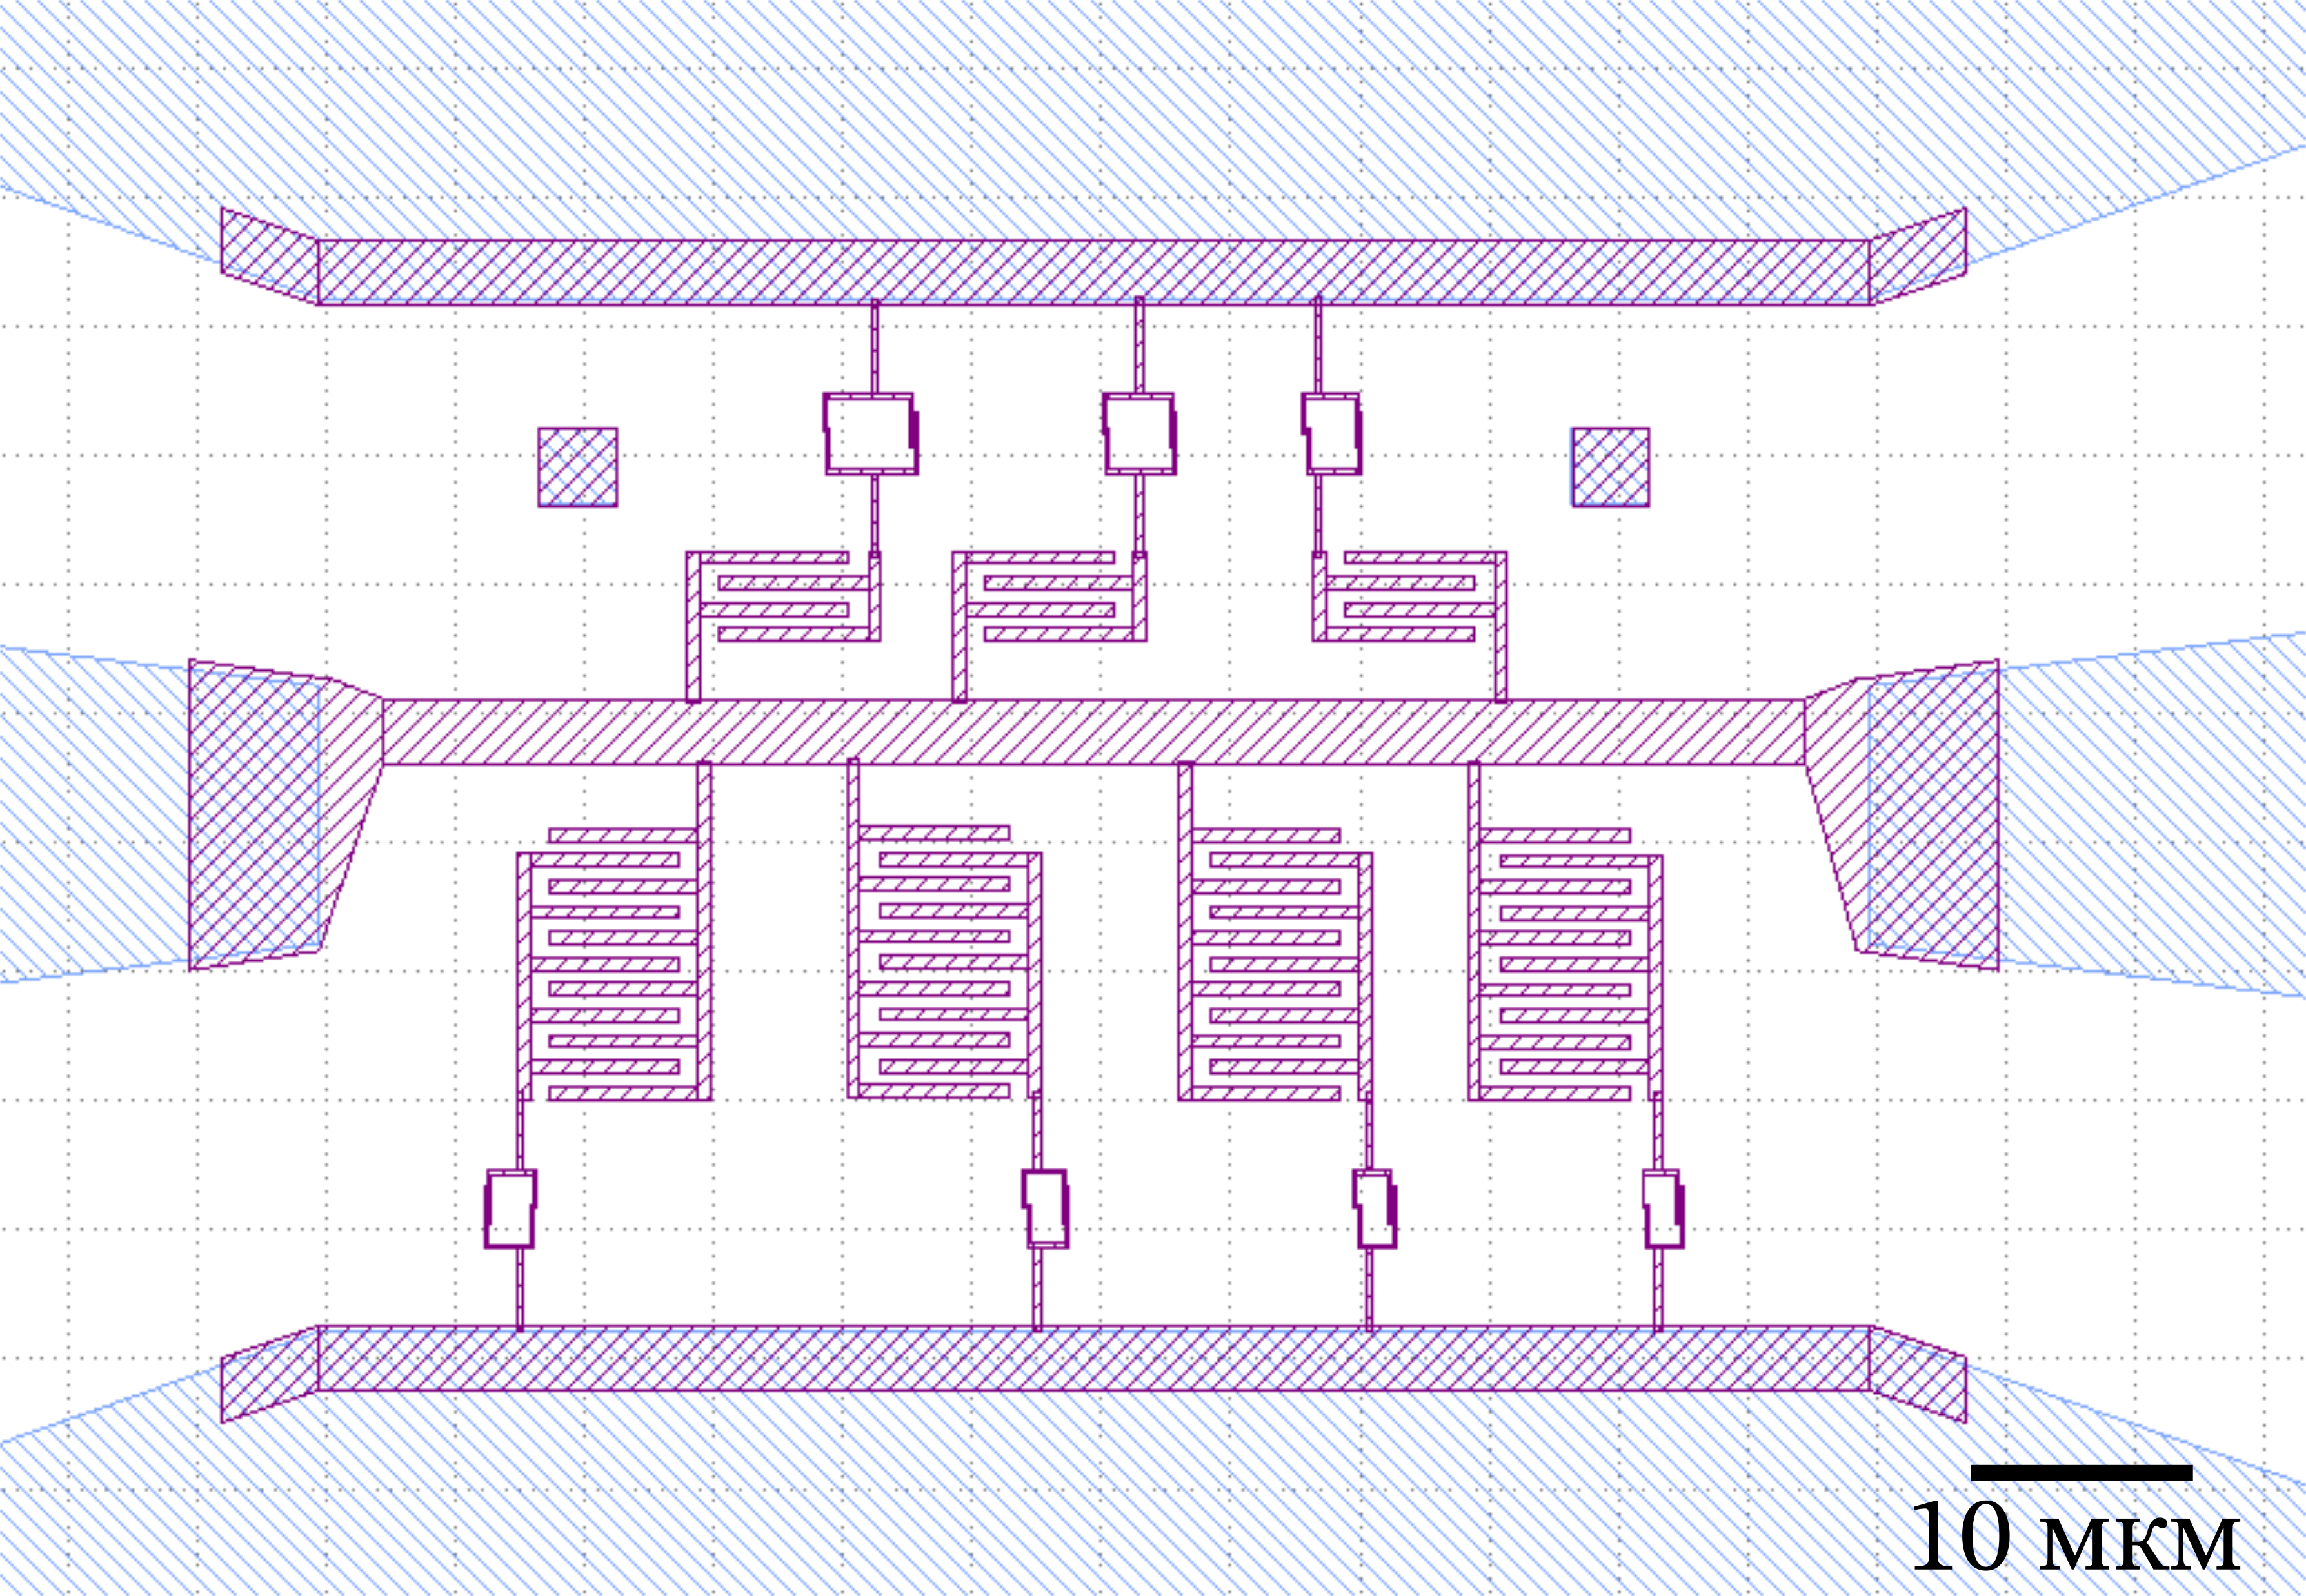
\includegraphics[width=0.7\textwidth]{ch_2/fig_qubits_2.png} \hfill
	\caption[width=0.6\textwidth]{Дизайн потоковых кубитов, емкостно связанных с копланарной линией. Параметр $\alpha=0.36,0.45$, площади петель от 5 до 40 мкм$^2$, связывающие емкости $C_c=2.2,6.4$~фФ }
	\label{fig: qubits_cap}
\end{figure}

Для последующей фабрикации были рассчитаны и отрисованы дизайны экспериментальные образцов: дизайн на рис. \ref{fig: qubits_sps} реализует режим прямой связи (англ. \textit{direct coupling}), а дизайн образца на рис.
\ref{fig: qubits_cap} --- режим параллельной связи (англ. \textit{side coupling}) кубита к излучению, однако, это различие не оказывает непосредственного влияния на спектры кубитов. Спроектированные дизайны содержат кубиты с 4-мя джозефсоновскими переходами, три из которых имеют одинаковую площадь $200\times800$~нм, а еще один переход в $\alpha\approx0.4$ раз меньше остальных. В этих схемах, кубит связывается с с электромагнитным полем, распространяющемся в копланарном волноводе, посредством связывающей емкости $C_c=2.2$-$6.4$~фФ, которая также оказывает шунтирующий эффект, необходимый для уменьшения чувствительности потокового кубита как к потоковым, так и зарядовым шумам.

\begin{figure}[htb]\center
	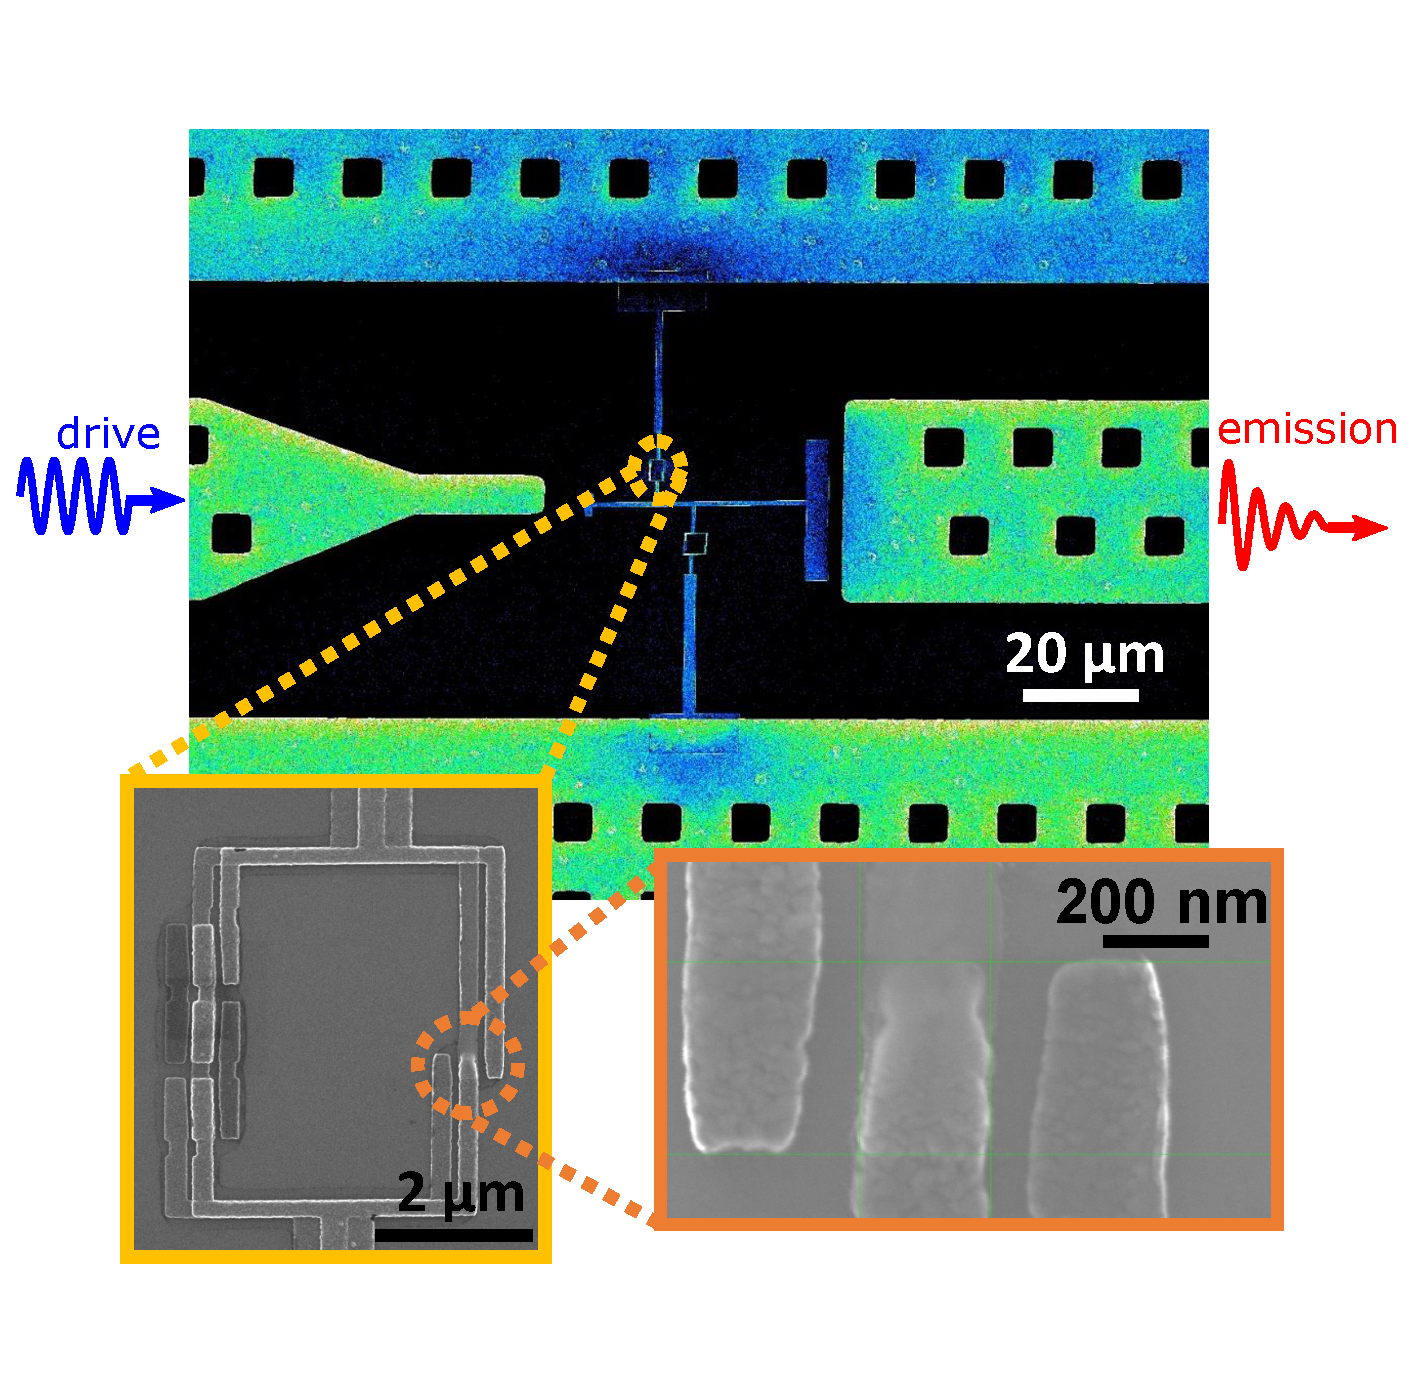
\includegraphics[width=0.7\textwidth]{ch_2/figure_1f.eps} \hfill
	\caption[width=0.6\textwidth]{Дизайн потоковых кубитов, емкостно связанных с копланарной линией по способу прямой связи. Параметр $\alpha=0.36,0.45$, площади петель от 5 до 40 мкм$^2$, связывающие емкости $C_c,C_e =0.5,5.5$~фФ }
	\label{fig: qubits_sps}
\end{figure}

Шунтирование~$\alpha$-перехода, добавляясь к внутренней емкости перехода $C_j=2$-$3$~фФ, уменьшает зарядовую энергию. Это необходимо для того, чтоб при тех же частотах кубита иметь возможность уменьшить джозефсоновские энергии переходов, что приведет к меньшей чувствительности кубита к магнитному полю и, соответсвеннно, к шуму магнитного потока, что при прочих равных условиях может увеличить время когерентности.. Влияние емкостного шунта на потоковые кубиты детально исследовано в работе \cite{yan2016flux}, как теоретически, так и экспериментально. При существенно б$\acute{\text{о}}$льших значений порядка $50$ фФ кубит, фактически, становится слабо ангармоничным осциллятором с небольшими следами <<двухъямности>>, ангармонизм падает ниже 1 ГГц, что нежелательно для выполнения поставленных в диссертации задач. Для иллюстрации изложенных закономерностей, на рис. \ref{fig: 3jj_spectra} приведены типичные зависимости энергии уровней от внешнего магнитного поля (спектры) кубитов для различных наборов параметров, полученные при помощи численной диагонализации полного гамильтониана. В рабочем режиме частота кубита $\omega_0=E_e-E_g/\hbar$ должна находиться в пределах 2-10 ГГц, что обусловлено частотными диапазонами криогенных усилителей и изоляторов (подробнее об этом ниже).

\begin{figure}[htb]\center
	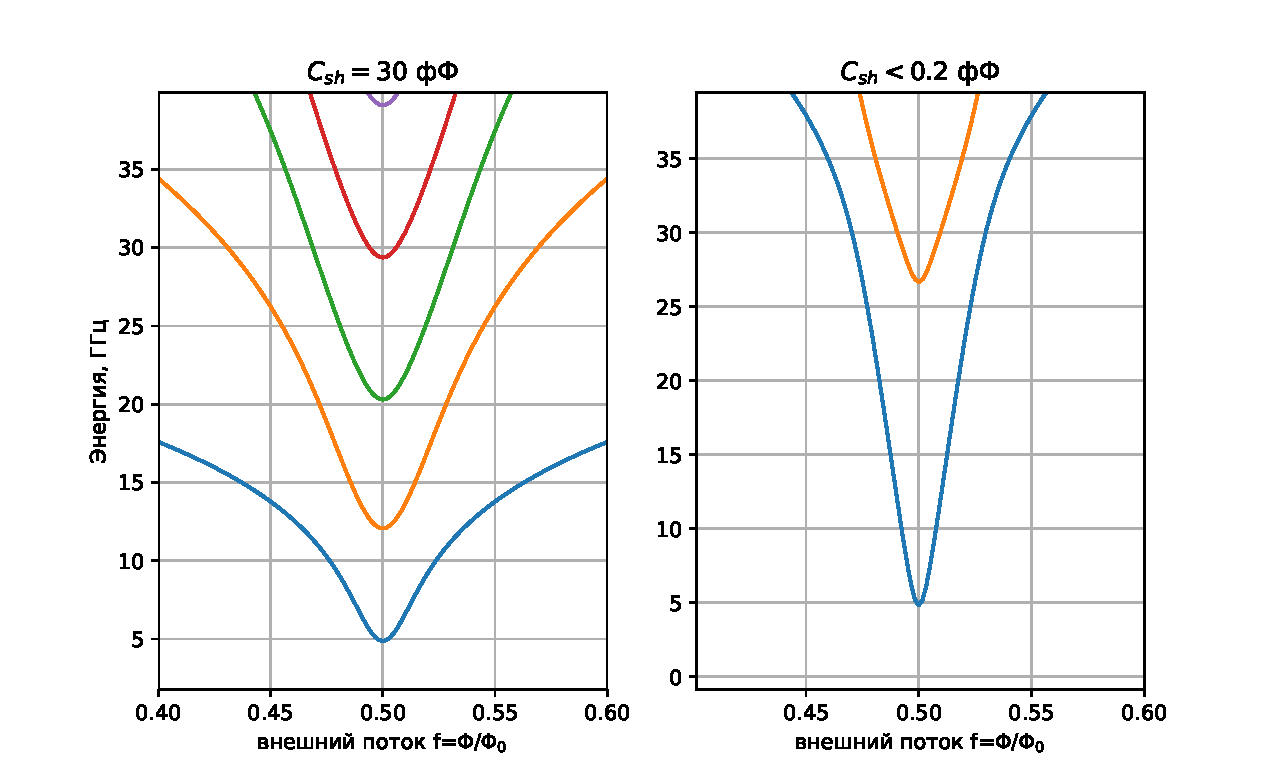
\includegraphics[width=1\textwidth]{ch_2/3jj_spectra.pdf} \hfill
	\caption[width=0.8\textwidth]{Рассчитанные спектры $E_n-E_0$ потоковых кубитов с тремя джозефсоновскими переходами с учетом влияния шунтирующей емкости $C_{sh}$ на $\alpha$-переходе. В обоих случаях $E_c = 25$~ГГц, $E_j=170$~ГГц. Левая панель: спектр для параметров $C_{sh} = 30$~фФ, $\alpha=0.5$. Правая панель: спектр для параметров $C_{sh} \approx 0.1$~фФ, $\alpha=0.69$. Как можно заметить, при равных параметрах переходов (что соответствует одинаковому процессу окисления) большая шунтирующая емкость сглаживает спектр и делает кубит не столь чувствительным к дефазировке по потоку, при этом ангармонизм еще достаточно велик (1-2 ГГц). В случае отсутствия шунта, приходится понижать частоту перехода 0-1 при помощи увеличения $\alpha$, однако, при смещении от оптимальной точки $f=0.5$ производная энергии по потоку слишком велика, и такой кубит гораздо сильнее подвержен дефазировке. Кроме того, при отсутствии шунта верхние уровни имеют слишком высокую частоту и недоступны для использования.}
	\label{fig: 3jj_spectra}
\end{figure}

Еще один важный аспект проектирования кубита заключается в том, что для наблюдения квантовооптических эффектов необходим режим сильной связи кубита и излучения, который можно определить следующим образом: безызлучательная релаксация $\Gamma_1^{nr}$ и чистая дефазировка $\gamma$ должны быть пренебрежимо малы по сравнению с константой связи (радиационной релаксацией)~$\Gamma^r_1$:
\begin{equation}
\Gamma^{nr}_1,\gamma \ll 
\Gamma_1^r = 2eV_{zpf}\cdot\beta\cdot\bra{g}\hat{N}_c \ket{e},
\label{eq:strong_c}
\end{equation} 
в случае емкостной связи. Здесь $V_{zpf}$ -- амплитуда вакуумных флуктуаций напряжения сигнала в линии, $\beta\approx \frac{C_c}{C_{\Sigma}}$ -- коэффициент пересчета, определяющий эффективное напряжение драйва и зависящий от емкостной части схемы кубита, $\hat{N_c}$ -- оператор связи, который определяется подключением кубита к внешнему полю и выражается некоторой комбинацией зарядовых операторов на островах кубита; например, для схемы с тремя джозефсоновскими переходами из \cite{yan2016flux} имеем $\hat{N}_c = \hat{n}_1 - \hat{n}_2$. Экспериментально известно, что при текущем уровне технологии $\Gamma_1^{nr}$ не превышает 1-2 МГц и возникает по причине двухуровневых систем в остаточном слое SiO$_2$ на поверхностях раздела подложки и металла, подложки и вакуума. Эта оценка показывает, что для достижения режима сильной связи достаточно иметь $\Gamma_1^r > 10$~МГц. Более точно режим сильной связи определяется в процесе экспериментов по измерению когерентного рассеяния, о которых будет сказано далее. 

Также в этом разделе описывается процедура фабрикации образцов. При изготовлении использовались распространенные методы фабрикации наноструктур из тонких пленок: электронно лучевая литография для структур с размерами более 50 нм, лазерная литография для структур с размерами более 3-4 мкм. Технические детали по отработке технологических параметров литографических и напылительных процессов (типы и толщины резистов, времена засветки, температуры, дозы, параметры проявления и смытия резиста) изложены в тексте диссертации, здесь же перейдем сразу к описанию процесса. Подложка из высокоомного недопированного кремния ($\rho$ = 10 кОм/cм) очищается при помощи стардартных процессов, широкоиспользуемых в кремниевой электронике: используются плавиковая кислота, кислородная плазма, RCA-1, RCA-2. После этого, наносятся фоточувствительные резисты LOR/S1813 и выполняется оптическая литография по предварительно загруженному дизайну в формате .gds. Затем, после проявления литографии напыляется копланарный волновод. Двухслойная маска в данном случае необходима для того, чтоб сформировать правильный профиль резиста в местах стыка непроявленной и проявленной части, и таким образом, избежать отрыва напыленной пленки в процессе <<взрывания>> маски (англ. \textit{lift-off}). Размеры центральной лини и зазоров контролируются при помощт оптического микроскопа, см. Рис. \ref{fig: line}. Электронная литография делается на двухслойной маске Copolymer/ARP-6200.04 с совмещением по меткам, затем засветка проявляется. Копланарная линия и кубит состоят из алюминия, напыляемого установкой электронно-лучевого напыления Plassys. Для этого образец загружается в камеру установки, и через полученную маску под углами $\pm$10-12\textdegree~напыляются алюминиевые пленки толщинами 25 и 45 нм соответственно, формирующие кубит и емкость. Между этими двумя напылениями в камеру с образцом напускается чистый кислород, и путем окисления верхней поверхности первой пленки происходит формирование туннельного барьера из аморфного оксида алюминия AlOx толщиной 2-3 нм, который впоследствии накрывается верхней пленкой при втором напылении; все это происходит в одном вакуумном цикле.  Типичные значения давления окисления для переходов  $p=$~1-2~мБар, что дает джозефсоновские энергии порядка 60-70~ГГц. После этого маска <<взрывается>>, и мы имеем готовую структуру. Затем необходимо измерить сопротивления тестовых джозефсоновских переходов, расположенных на этом же чипе, напыленных в том же вакуумном цикле что и кубиты и имеющих контактные площадки для подведения к ним зондов измерительной станции. Это делается для предварительной оценки джозефсоновской энергии. Затем образец покрывается защитным слоем резиста, распиливается под формат печатной платы с помощью дисковой пилы, после чего резист смывается и происходит финальная отмывка подложки. По данному рецепту было изготовлено несколько чипов с потоковыми кубитами в линии, см. Рис. \ref{fig: qubits}. 

\begin{figure}[htb]\center
	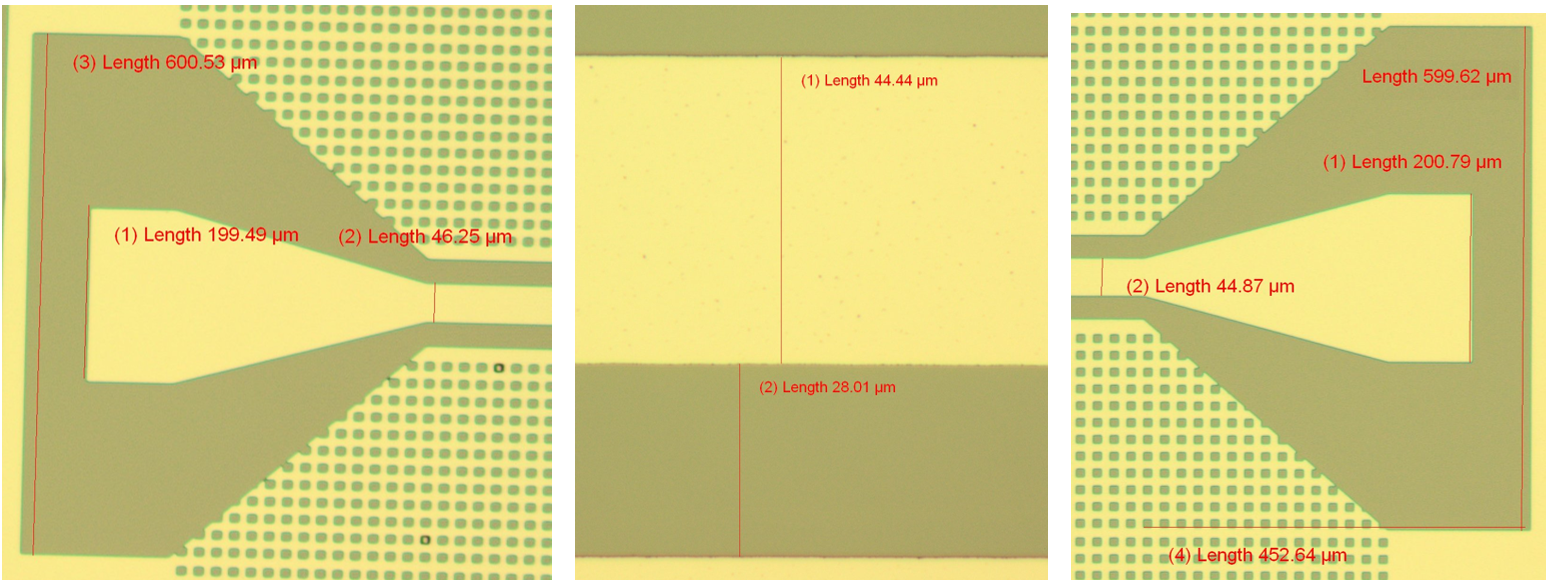
\includegraphics[width=1\textwidth]{ch_2/line_opt_control.png} \hfill
	\caption[width=0.6\textwidth]{Контроль продольных и поперечных размеров копланарной линии при помощи оптического микроскопа}
	\label{fig: line}
\end{figure}

\begin{figure}[htb]\center
	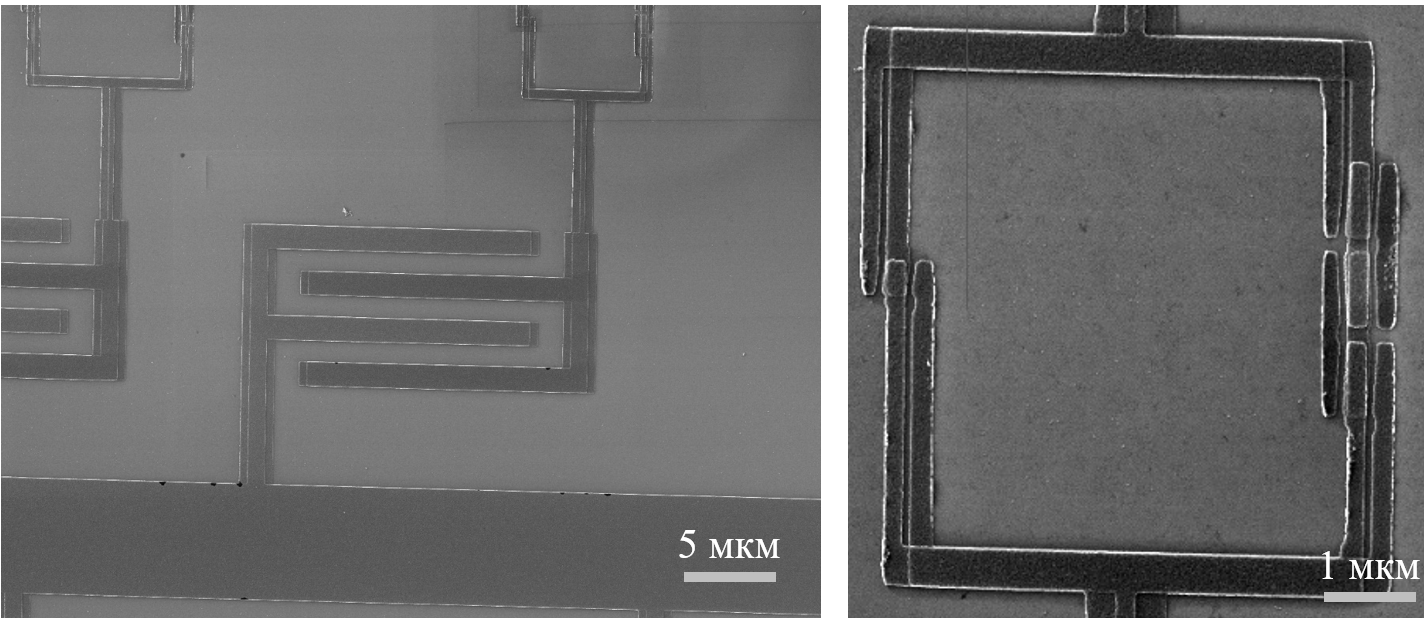
\includegraphics[width=1\textwidth]{ch_2/qubits.png} \hfill
	\caption[width=0.6\textwidth]{Связывающая емкость и кубит. Изображение сделано прои помощи электронного микроскопа}
	\label{fig: qubits}
\end{figure}
\textbf{Раздел 2.2} описывает измерительную схему, необходимую для характеризации кубитов. Для того, чтоб иметь возможность работать со сверхпроводящим кубитом, сильно связанным с модами копланарой линии, необходимо выполнить ряд условий.
Первое и самое очевидное: характерная энергия перехода кубита $\ket{g} \leftrightarrow \ket{e}$ составляет $\omega_{eg}=6\cdot 10^{9}$~Гц $\sim 300$~мК, и поэтому для квантовости системы ее необходимо охладить до гораздо более низких температур. Для этого кубит помещается в медный держатель, прикрепляемый на нижнюю ступень криостата растворения с базовой температурой 15 мК.

Далее, для возбуждения и измерения кубита необходимо подвести к нему высокочастотный сигнал от генератора либо анализатора цепей. Для этого используются коаксиальные кабели, которые при помощи специальных разъемов выводятся на копланарные линии печатной платы, в которой имеется прорезь для размещения кремнивого чипа с кубитом. Высокочастотный сигнал, доведенный до линии на печатной плате, необходимо далее передать в волновод с кубитом без потерь и отражений, насколько это возможно. Для этого используется специальная машина ультразвуковой микросварки, которая позволяет гальванически соединить контактные площадки на чипе с сигнальными линиям на печатной плате при помощи отрезков тонкой алюминиевой проволоки с толщиной 25 мкм, привариваемых к чипу и к плате. При этом, на частоте 6 Ггц данная проволока имеет заметную индуктивность: для отрезка длиной 300 мкм имеем $L=0.2$~нГ, что дает импеданс $Z = \omega L= 13.56$~Ом, сравнимый с волновым сопротивлением линии в 50 Ом. Поэтому, дабы не вносить отражений из-за сосредоточенного импеданса, сигнальные линии стараются приваривать на чип как минимум 3-4 отрезками проволоки (англ. \textit{wire bonds}).

Еще одна сложность состоит в том, что любой провод, идущий от комнатной температуры на чип, также будет прекрасным проводником равновесных тепловых фотонов, которые, распространяясь от фланцев криостата с более высокими температурами, будут сильно нагревать чип. Для этого на входные линии помещается определенное количество атенюаторов. Суммарное ослабление в них можно в первом приближении оценить исходя из формулы Джонсона-Найквиста для спектральной плотности теплового шума: $A[\text{Дб}]=10\log_{10}(T_r/T_{cold})$, при этом ослабление должно распределяться по фланцам равномерно с уменьшением температуры, чтобы температура излучения, распространяющегося с верхних, более горячих ступеней, после ослабления примерно соответствовала равновесной температуре излучения в том аттенюаторе, который и ослабил напряжение от фотонов.  

Прежде всего, нас будут интересовать режимы, в которых сигнал, излучаемый или рассеиваемый кубитом, чрезвычайно мал, поэтому для детектирования  его необходимо усилить. Сигнал имеет очень низкую мощность, порядка $10^{-16}$~Вт, поэтому необходим низкотемпературный высокочастотный усилитель с ультранизким уровнем шумов, $T_{noise} \sim 5$-$10$~K. В то же время, тепловой шум в этих линиях также нужно ослаблять, поэтому непосредственно перед усилителем в линию включается важный элемент --- изолятор, служащий диодом для высокочастотного сигнала. 

Как известно, энергия состояний потокового кубита зависит от величины внешнего магнитного потока $\Phi_{ext}$. Удобно иметь возможность выбирать рабочую точку, меняя частоту, поэтому необходимо предусмотреть возможность создавать стабильное магнитное поле через петлю кубита, и обеспечивать его плавное изменение без рассеивания тепла --- для этого держатель с образцом помещается внутрь сверхпроводящей катушки. 
Приняв во внимание все вышеперечисленное, была спроектированы и собраны схемы для измерений кубита, см. Рис \ref{fig: schemes}. Можно отметить, что схемы отличаются для различных типов каплинга, поскольку техника проведения измерений, и как следствие, измеряемые величины несколько различны, о чем будет более подробно рассказано в следующеем разделе.

\begin{figure}[htb]\center
	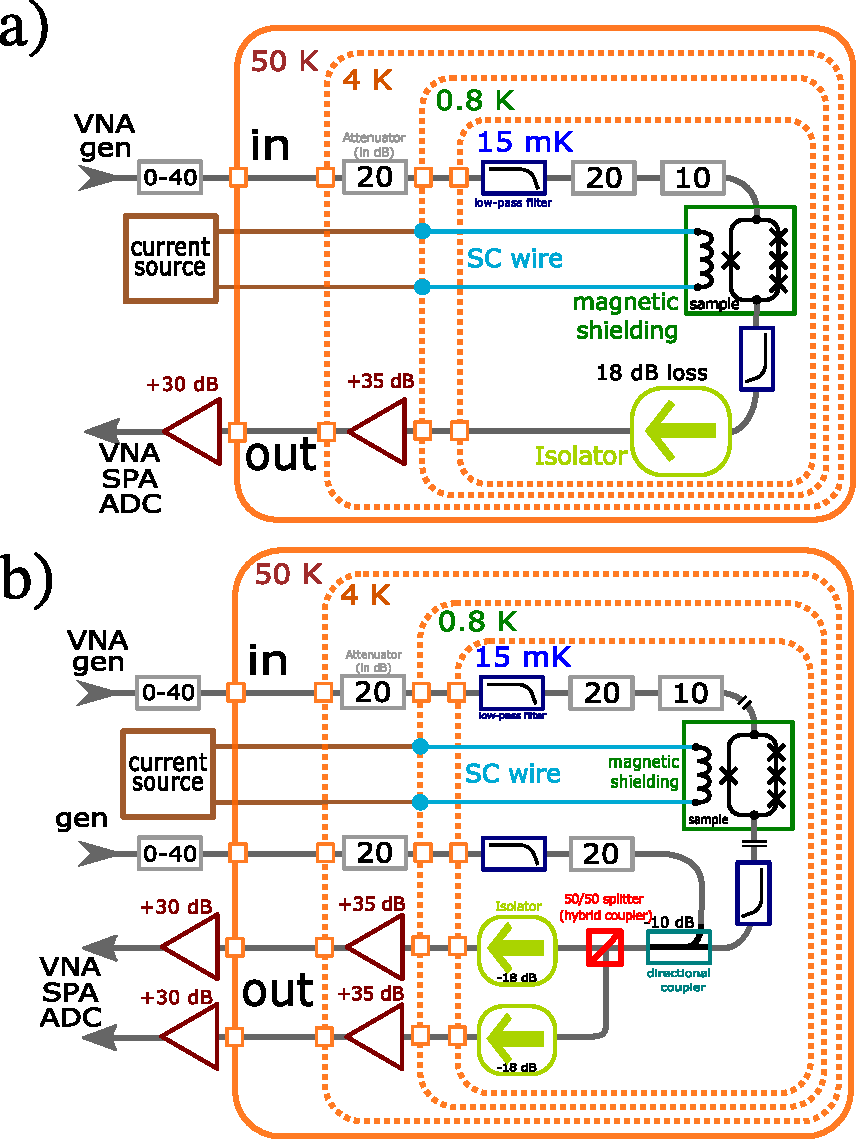
\includegraphics[width=0.8\textwidth]{ch_2/meas_schemes_2.pdf} \hfill
	\caption[width=0.6\textwidth]{Низкотемпературная часть измерительных схем. а) --- схема для кубита в линии (параллельная связь), б) --- схема для кубита, связанного с двумя полупространствами (прямая связь) }
	\label{fig: schemes}
\end{figure}

\textbf{Раздел 2.3} представляет результаты спектроскопических измерений кубитов в линии, в частности, эластичного и неэластичного рассеяния. Измерительная схема для случая параллельной связи дает возможность изучать данную систему, посылая микроволновое излучение от векторного анализатора цепей в линию и детектируя амплитуду и фазу когерентной части прошедшего сигнала. Таким образом можно измерить относительный коэффициент прохождения $t=V/V_0$ непрерывной волны (англ. \textit{continious wave}) через линию c кубитом. Аналитическое выражение для прохождения в линии с учетом взаимодействия волны и кубита может быть получено при решении основного квантового уравнения (англ. \textit{quantum master equation}) для двухуровневой системы в форме Линдблада: 
\begin{equation}
\dot{\rho}=-\frac{i}{\hbar}[\hat{H},\rho] + 
\begin{pmatrix}
-\Gamma_1 (1-\rho_{gg})& -\Gamma_2 \rho_{eg}\\
-\Gamma_2 \rho_{eg}&\Gamma_1 \rho_{gg}
\end{pmatrix}
\label{eq:master}
\end{equation}
Где гамильтониан $\hat{H} = (-\delta\omega\hat{\sigma}_z -\Omega\hat{\sigma}_x)/2$ записан в приближении вращающейся волны. В результате поиска стационарного решения $\dot{\rho}=0$~получается следующее выражение для коэффициента отражения:
\begin{equation}
r = 1-t = \frac{\Gamma_1}{2\Gamma_2}\frac{1+i\delta\omega/\Gamma_2}{1+(\delta\omega/\Gamma_2)^2 + \Omega^2/\Gamma_1\Gamma_2},
\label{eq:refl}
\end{equation}
где $\Gamma_1$ и $\Gamma_2$ --- скорости релаксации и дефазировки, соответственно. Измеренные зависимости $t$ от частоты для различных кубитов изображены на Рис. \ref{fig: refl_fit} и хорошо согласуются с соотношением \eqref{eq:refl}, что говорит о режиме сильной связи. Аппроксимируя экспериментальную кривую, полученную в режиме малой амплитуды, когда $\Omega \ll \Gamma_1, \Gamma_2$, можно определить $\Gamma_1$ и $\Gamma_2$ для  кубита при фиксированном внешнем потоке. Данные этих измерений представлены в табл. \ref{table}.
\begin{table} [htbp]
	\centering
	\changecaptionwidth\captionwidth{14cm}
	\caption{Параметры кубитов. Эффективность отражения (англ. \textit{extinction}), $\Gamma_{1},\Gamma_2$~измерены в точке вырождения.}\label{table}%
	\begin{tabular}{| p{0.8cm} || p{0.8cm} | p{0.8cm} | p{0.8cm} | p{0.8cm} | p{0.6cm}l |}
		\hline
		\hline
		\centering№ кб. & \centering $\nu_{deg}$, ГГц & \centering $C_{sh}$, фФ & \centering эфф. отр. & \centering $\Gamma_1$, МГц &\centering  $\Gamma_2$, МГц & \\
		\hline	
		\centering1 &\centering  5.75  &\centering  1  &\centering   0.85  &\centering   1.56 &\centering   1.55 &   \\
		\centering2  &\centering  6.17  &\centering  2  &\centering   0.97 &\centering   2.20 &\centering   1.40  &   \\
		\centering3 &\centering  5.85  &\centering  2.5  &\centering  0.95 &\centering   2.62 &\centering   1.99  &   \\
		\centering4 &\centering  5.82  &\centering  3  &\centering   0.94 &\centering   1.96 &\centering   0.98  &   \\
		\centering5 &\centering  5.26  &\centering  3.5  &\centering   0.95 &\centering   3.99 &\centering   2.94  &   \\
		\hline
		\hline
	\end{tabular}

\end{table}

Практически для всех образцов выполняется сотношение $\Gamma_2 = \Gamma_1/2$, что свидетельствует о пренебрежимо малом значении чистой дефазировки.
 
\begin{figure}[htb]\center
	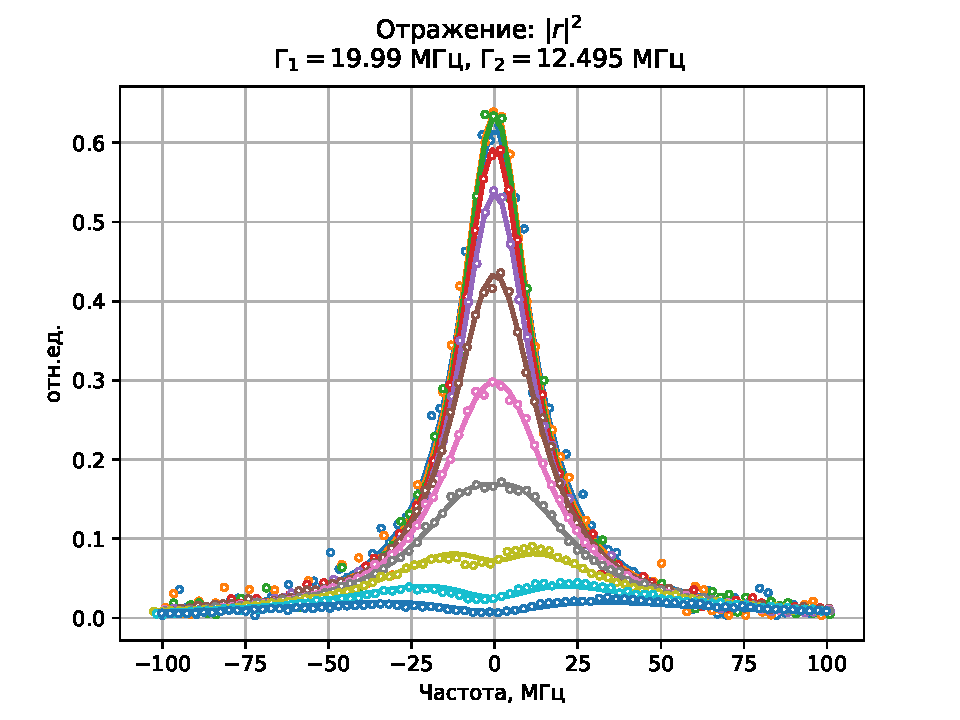
\includegraphics[width=0.8\textwidth]{ch_2/line_fit.pdf} \hfill
	\caption[width=0.6\textwidth]{Результаты измерений коэффициента резонансного отражения $R=|r|^2$ для потокового кубита, при помощи подгонки данных формулой \eqref{eq:refl} получены параметры $\Gamma_1/2\pi$ и $\Gamma_2/2\pi$ }
	\label{fig: refl_fit}
\end{figure}

В \textbf{разделе 2.4} представлены результаты измерения спектра резонансной флуоресценции. Еще один способ, позволяющий измерить релаксацию и дефазировку - измерение некогерентной части рассеянного сигнала на кубите, т.н. \textit{резонансной флуоресценции} \cite{Astafiev2010resonance,Mollow}. Поскольку для когерентного сигнала $t+r=1$, то для мощностных коэффициентов прохождения $T=|t|^2$ и отражения $R=|r|^2$ выполнено $T+R <1$. Это значит, что часть мощности рассеивается некогерентно, с изменением частоты и фазы, и доля этой некогерентной части излучения возрастает при увеличении $\Omega$.  Это излучение можно обнаружить при помощи спектрального анализатора с широкой полосой входного фильтра (>1 МГц) при достаточно большом усреднении. Спектральная плотность излучения флуоресценции может быть рассчитана с использованием теоремы Винера-Хинчина и квантовой регрессионной теоремы. Окончательный ответ \cite{Astafiev2010resonance, abdumalikov2011dynamics} имеет вид:
\begin{equation}
S(\omega) = \frac{1}{2\pi}\frac{\hbar \omega\Gamma_1}{8}\Big(\frac{\gamma_s}{(\delta\omega+\Omega)^2+\gamma_s^2}+\frac{2\gamma_c}{\delta\omega^2+\gamma_c^2}+\frac{\gamma_s}{(\delta\omega-\Omega)^2+\gamma_s^2}\Big).
\label{eq: mollow}
\end{equation}
Результаты измерений для случая $\delta\omega$ хорошо соответствуют этой зависимости, см. рис. \ref{fig: mollow} .  Из этой аппроксимации определяются параметры $\Gamma_1$~и~$\Gamma_2$ и амплитуда драйва $\Omega$. Результаты для этих величин также согласуются с измерениями коэффициентов резонансного (когерентного) пропускания.  
%соотвествующей когерентному состоянию $\ket{\alpha}$ cо средним чиcлом фотонов  $\bar{n}=|\alpha|^2 \ll 1$ (то есть, волны с %достаточно малой амлитудой), происходит полное отражение волны: $r=1$, см.~Рис. \dots . 
\begin{figure}[htb]\center
	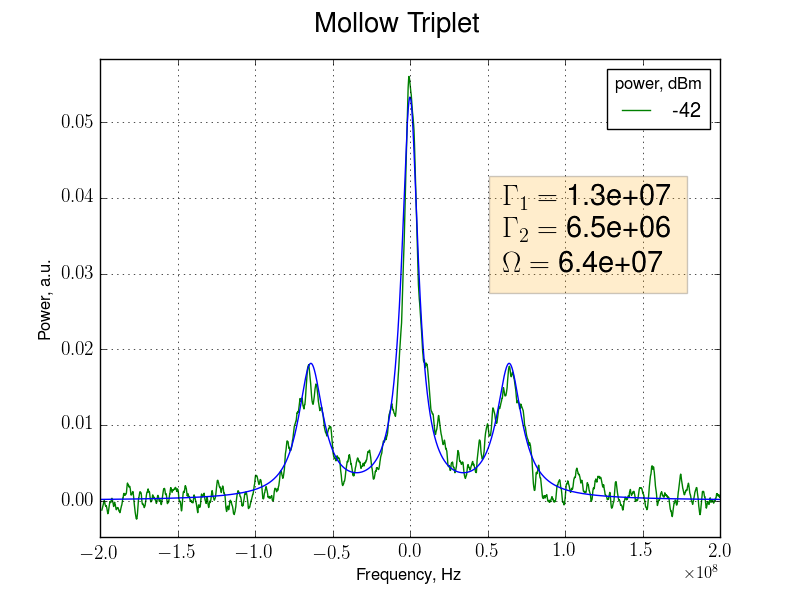
\includegraphics[width=0.6\textwidth]{ch_2/Mollow_Triplet_fit.png} \hfill
	\caption[width=0.6\textwidth]{Результаты измерений спектра некогерентного рассеяния для потокового кубита. При помощи подгонки данных формулой \eqref{eq: mollow} получены параметры $\Gamma_1/2\pi$, $\Gamma_2/2\pi$ и $\Omega/2\pi$ }
	\label{fig: mollow}
\end{figure}

\textbf{Раздел 2.5} представляет результаты импульсных измерений динамики одиночных потоковых кубитов в линии. Для отладки импульсных методик и их использования для приготовления квантовых состояний собиралась и тестировалась схема, принципиальный вид которой отображен на рис.~\ref{fig: time_domain}. Приготовление квантовых состояний кубита осуществляется при помощи микроволновых смесителей с рабочими частотами 4-9 ГГц и генераторов сигналов произвольной формы с полосой $330$~МГц и частотой отсчета 2 ГГц. На выходе схемы формируются прямоугольные либо гауссовские цуги высокочастотного сигнала, с периодом $\sim$ 10 МГц, которые затем посылаются в линию с кубитом. Длительность цуга определяет квантовое состояние, в котором оказывается кубит после прохождения цуга. Рассеянный сигнал пропукается через считывающую цепь, и выделяется когерентное излучение кубита, распространяющееся в линии сразу после возбуждения, по которому можно восстановить квантовое состояние. В частности, схема позвояет реализовать Раби экперимент, см. Рис.~\ref{fig:qosc}, а также измерить свободную дефазировку, см. Рис.~\ref{fig:g2}. Характерное время затухания Раби осцилляций  $T_R \approx 4/3\cdot T_1$ составляет 30-50 нс, что соответствует измеренным ранее $\Gamma_1$. 

\begin{figure}[htb]\center
	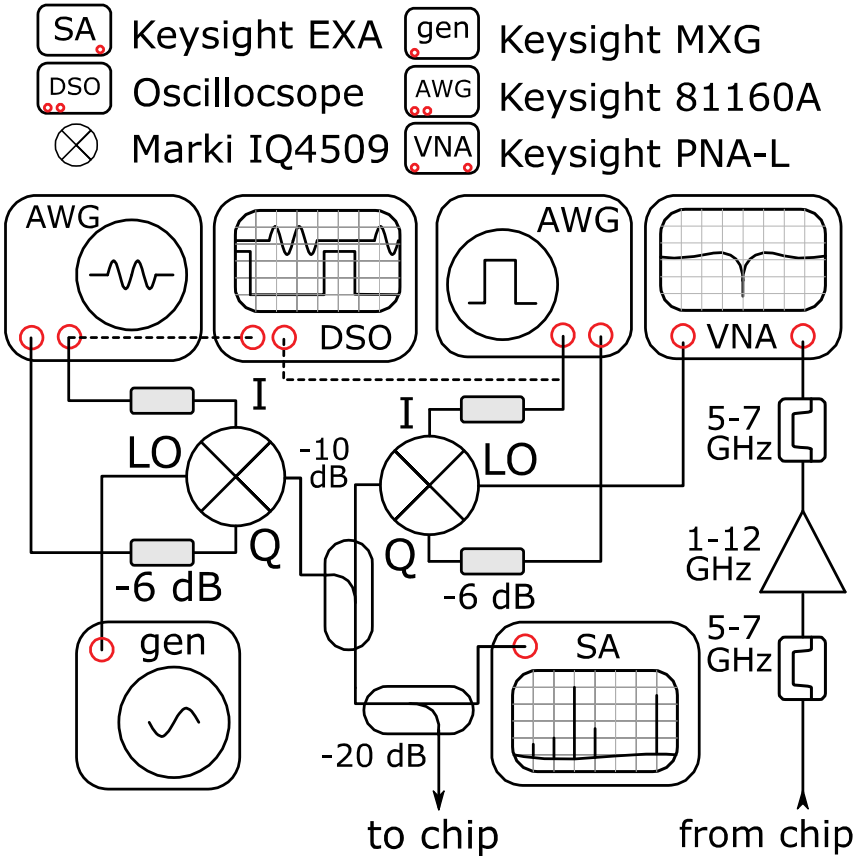
\includegraphics[width=0.5\textwidth]{ch_2/scheme.png} \hfill
	\caption[width=0.6\textwidth]{Обобщенный вариант измерительной схемы для управления и контроля состояний кубитов в линии.}
	\label{fig: time_domain}
\end{figure}

\begin{figure}[thb]\center
	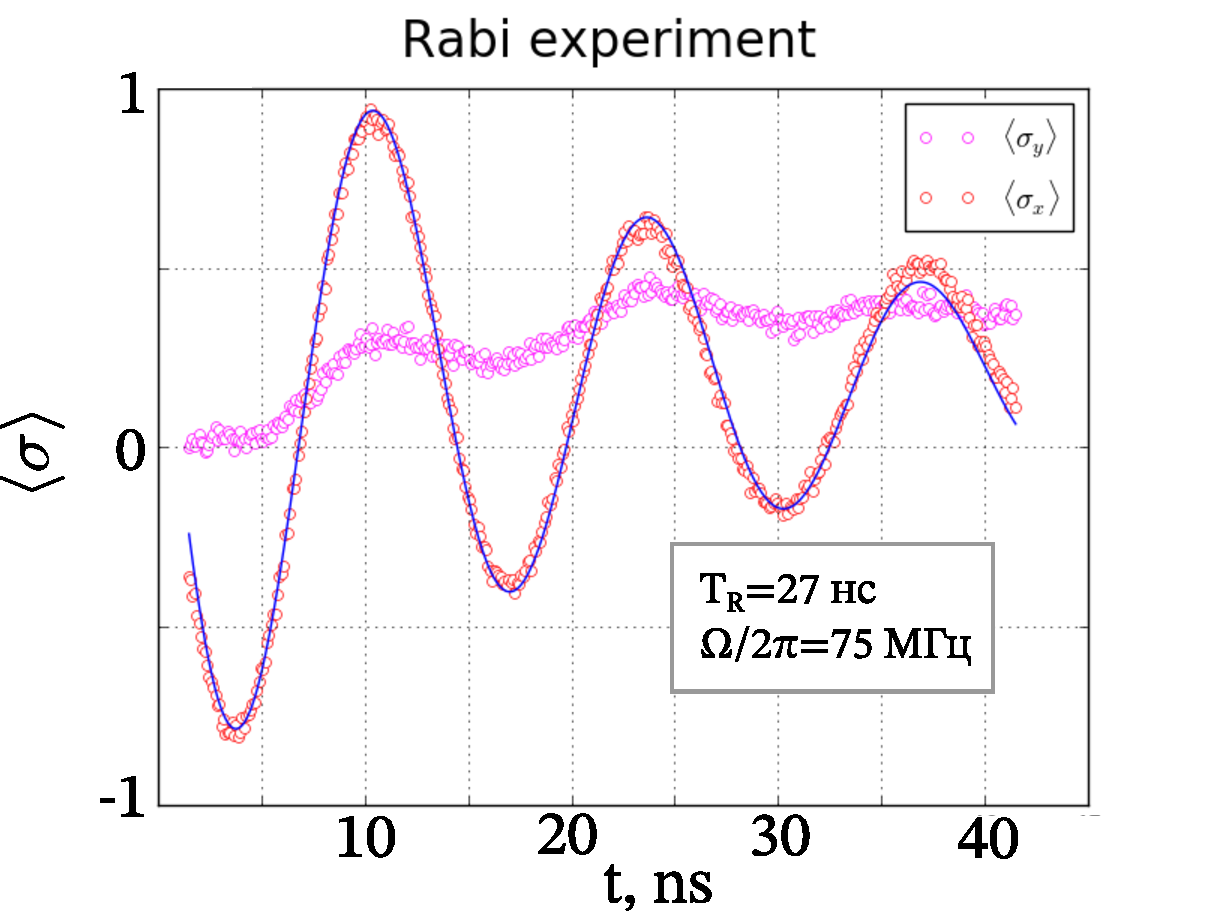
\includegraphics[width=0.6\textwidth]{ch_2/Rabi.pdf}
	\caption{Раби-осцилляции для потокового кубита: среднее значение квадратуры рассеянного когерентнго сигнала соответствует заселенности кубита. Из параметров подгоночной кривой	можно определить время Раби и амплитуду возбуждения (в линейных единицах частоты)}
	\label{fig:qosc}
\end{figure}
Практический интерес представляет также схема, в которой кубит неодинаково связан с двумя разделенными полупространствами, см. Рис. \ref{fig: qubits_sps}, спектры которого изображены на рис.~\ref{fig: spectra_sps}. Такая схема, например, позволяет отделить квантовое излучение кубита от классического поля, используемого для приготовления квантовых состояний кубита в линии. Хорошее пространственной согласование мод кубита и открытой линии приводит к тому, что любая квантовая суперпозиция кубита излучается в выходную линию, то есть если система <<атом-электромагнитное поле>>~приготовлена в  состоянии $(|g\rangle + e^{j\phi}|e\rangle \otimes |0\rangle)$, то через время релаксации она перейдет в состояние $|g\rangle \otimes (|0\rangle + e^{j\phi}|1\rangle)$, то есть, состояние электромагнитного поля будет квантовой суперпозицией, сохраняющей фазу состояния кубита. Если же приготовить кубит в возбужденном состоянии: $|e\rangle \otimes |0\rangle$, то при релаксации излучится один фотон. Если при этом одна из линий связана сильнее другой, то поле будет распространяться по ней в большинстве случаев --- получится генерация фотона по требованию \cite{peng2016tuneable}. Отметим также, что данная схема принципиально позволяет излучать детерминированным образом не только одиночные фотоны, но также любую квантовую суперпозицию вида $|0\rangle + e^{i\alpha}|1\rangle$, что практически невозможно, скажем, для оптического источника одиночных фотонов, основанного на спонтанном параметрическом рассеянии света в нелинейном кристалле \cite{grangier1986experimental}. Были изготовлены образцы кубитов с ассимметричными емкостями связи: $C_c=0.5$~фФ, $C_e=5$~фФ, при помощи многотоновой спектроскопии были определены частоты первых трех переходов кубита, установлено соответствие с численным расчетом спектра, см. Рис. \dots и определены параметры $E_c=$, $E_J=$, $\alpha=$. Также отсняты излучательные характеристики линий и показано расщепление Аутлера-Таунса (англ. \textit{Autler-Townes splitting}). 
\begin{figure}[htb]\center
	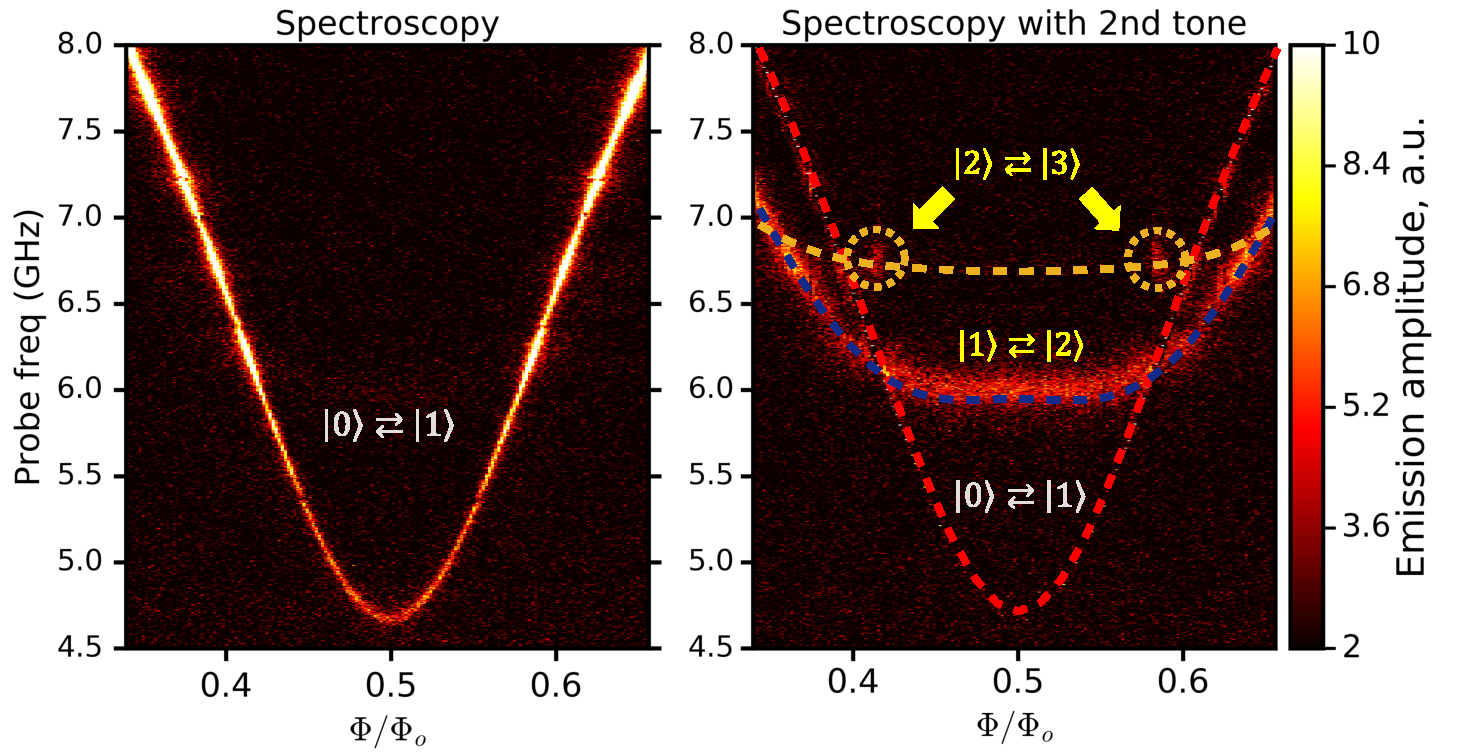
\includegraphics[width=0.7\textwidth]{ch_2/figure_2-1.pdf}
	\caption{Спектры энергий переходов кубита, связанного с двумя полупространствами. Слева изображен переход 0-1, возбуждаемый слабым сканирующим сигналом. Справа изображен спектр, получаемый при добавлении второго тона, резонансного с переходом 0-1, при этом проявляется спектральная линия перехода 1-2 и элементы перехода 2-3. Уровни энергии хорошо согласуется с рассчитанным при помощи диагонализации гамильтониана спектром.  }
	\label{fig: spectra_sps}
\end{figure}

% картинку можно добавить так:
%\begin{figure}[ht] 
%	\centering
%	\includegraphics [scale=0.27] {latex}
%	\caption{Подпись к картинке.} 
%	\label{img:latex}
%\end{figure}
%
%Формулы в строку без номера добавляются так:
%\[ 
%\lambda_{T_s} = K_x\frac{d{x}}{d{T_s}}, \qquad
%\lambda_{q_s} = K_x\frac{d{x}}{d{q_s}},
%\]

В \textbf{разделе 2.6} излагаются причины и предпосылки к наблюдению такого эффекта, как нелинейное смешивание волн, распространяющихся через линию со встроенным в нее искусственным атомом. Введем параметр $\zeta=\Omega/\Gamma_1$, и проанализируем зависимость выражения \eqref{eq:refl} от амплитуды внешнего поля $\Omega$ при $\delta\omega=0$.  Разложим выражение в ряд при $\zeta\ll1$ :
\begin{equation}
t \propto 1-\frac{1}{1+2\zeta^2} = 2\zeta^2 - 4\zeta^4 + ...
\label{eq:t_nonl}
\end{equation}
Мы видим, что в разложении присутствуют члены, пропорциональные степеням $\zeta^{2n}$ и возрастающие по мере увеличения $\Omega$, что эквивалентно появлению компонент электрической восприимчивости, пропорциональных нечетным степеням электрического поля, $\chi^{(2n+1)}E^{2n+1}$, в оптических средах. Однако, при больших амплитудах драйва, когда $\zeta\gg1$, выражение \eqref{eq:t_nonl}  принимает вид
\begin{equation}
t \propto \frac{1}{1+1/(2\zeta^{2})} = 1 - \frac{1}{2\zeta^2} + \frac{1}{4\zeta^4} - ... ,
\end{equation}
из чего следует, что при слишком больших амплитудах нелинейные эффекты вновь пропадают. Исходя из этого, можно ожидать проявления смешивания волн примерно в области $\zeta\approx1$.  Параметр $\zeta$ показывает, насколько атом способен, в силу своей двухуровневости, рассеивать внешнее поле, поскольку $\Omega$ представляет из себя скорость поглощения и испускания атомом одиночного фотона из когерентного сигнала, а $\Gamma_1$ --- скорость спонтанной эмиссии из возбужденного состояния. Также в этом разделе проводится сравнение эффективной нелинейности третьего порядка $\chi^{(3)}$ сверхпроводникового кубита и паров атомов гелия. Показано, что сверхпроводниковый кубит является гораздо более нелинейной системой за счет возможности изучения резонансного рассеяния. 

\underline{\textbf{Глава 3}} посвящена изучению смешивания двух когерентных резонансных волн на сверхпроводящем кубите. 

\textbf{Раздел 3.1} кратко описывает известные теоретические результаты по оптическому смешению в нелинейных средах, также приводятся причины, затрудняющие прямое применение традиционного формализма к исследуемому далее случаю смешения микроволн на кубите.

\textbf{Раздел 3.2} описывает теорию, при помощи которой рассчитывается спектр неэластичного рассеяния под действием бихроматической накачки. Отмечается, что в рамках существующих теоретических работ отсутствует результат для интенсивности когерентных компонент в случае, когда отстройка между сигналами накачки и резонансом атома пренебрежимо мала по сравнению с радиационной релаксацией кубита в открытое пространство. 

\textbf{Раздел 3.3} представляет результаты эксперимента по рассеянию двух когерентных волн на сверхпроводящем кубите. На кубит с частотой перехода $\omega_{ge}$ через входной тракт подается две непрерывные волны, полученные при помощи высокочастотных генераторов (Keysight MXG N5182A) и сведенные в один коаксиальный выход при помощи микроволнового расщепителя (англ. \textit{microwave splitter}). Частоты $\omega_+$ и $\omega_-$ выбираются так, чтобы $\omega_{ge}\approx\omega_-,\space\omega_+$ и $\omega_+-\omega_- \ll \Gamma_1$. При измерении спектров сигнала наблюдается следующая картина, см. рис. \ref{fig: fwm_qubit} : помимо исходных волн, в спектре возникает целый ряд гармоник с частотами $\omega_{\pm(2k+1)}=\pm(k+1)\omega_{\pm}\mp k\omega_{\mp}$, что свидетельствует о смешивании стационарных волн на одиночном искуссвенном атоме. Происхождение боковых спектральных компонент можно также пояснить, рассматривая многофотонные процессы рассеяния света, см. рис. \ref{fig: fwm_multphot}. Был проведен подробный экспериментальный анализ данного явления, в ходе которого получены зависимости интенсивности боковых спектральных компонент от мощности сигналов накачки $\Omega_+,\space\Omega_-$, от <<глобальной>> отстройки $\Delta\omega = \omega_{eg}-\omega_d$, где мы обозначаем $\omega_d\equiv(\omega_+-\omega_-)/2$, от локальной отстройки $\delta\omega$. Некоторые из этих зависимостей отображены на Рис. \dots. Они также сопровождаются подгоночными кривыми, полученными из теоретических соображений. 
\begin{figure}[htb]\center
	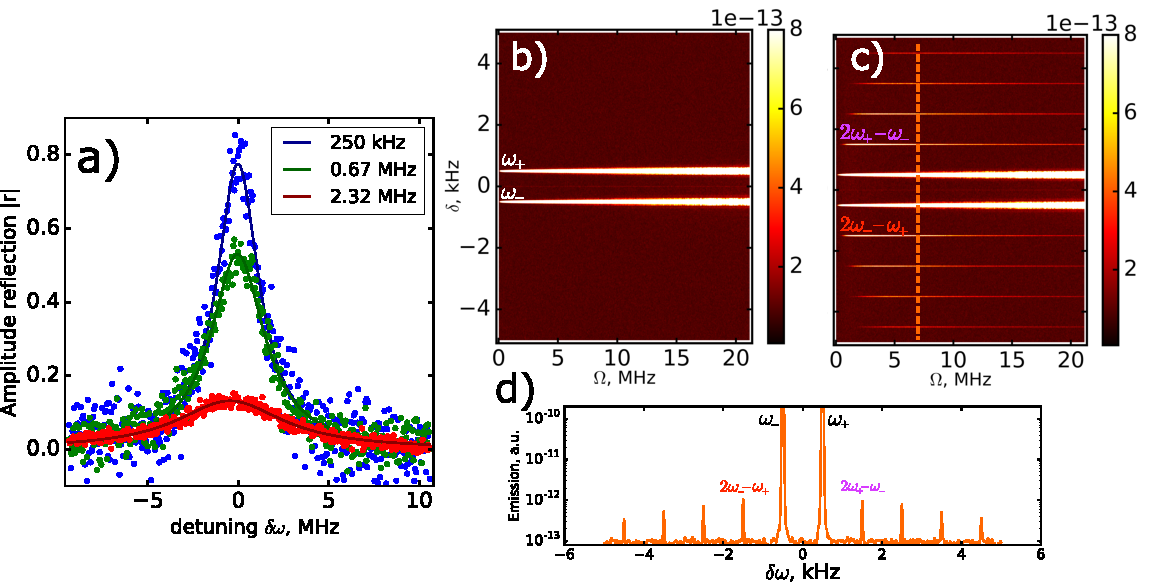
\includegraphics[width=0.9\textwidth]{ch_3/CWM_2_2-1.pdf}
	\caption{\textbf{(a)} Кубит, облучаемый непрерывным сигналом на резонансной частоте, рассеивает свет когерентным образом, что приводит к значительному отражению сигнала низкой мощности (синяя кривая). При увеличении мощности, переход насыщается и отражение уменьшается (зеленая и красная линии). \textbf{(b, c)} Спектры когерентного рассеяния двух близких по частоте сигналов (b) вне резонанса либо (c) в резонансе с кубитом, построенный как функция амплитуд обоих сигналов: $\Omega_+$=$\Omega_-$=$\Omega$. График \textbf{(d)} представляет измеренный спектральным анализатором график для фиксированной амплитуды.}
	\label{fig: fwm_qubit}
\end{figure}

\begin{figure}[htb]\center
	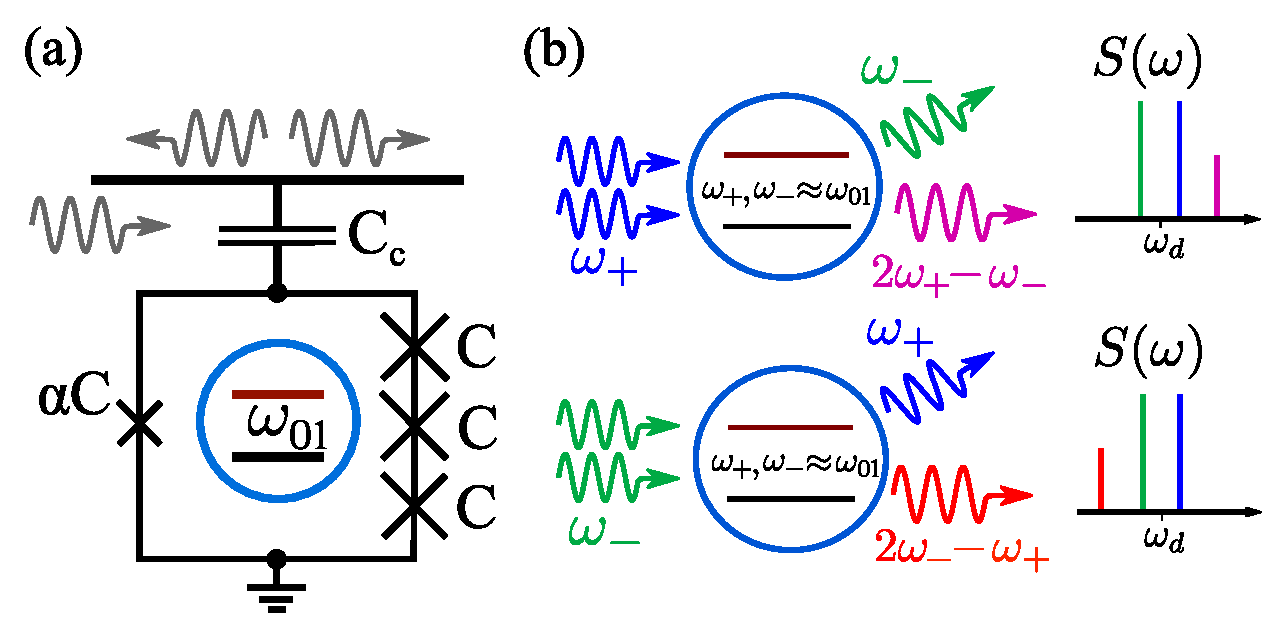
\includegraphics[width=0.7\textwidth]{ch_3/CWM_1-5.pdf}
	\caption{Смешивание волн на сверхпроводящем кубите с точки зрения многофотонных процессов рассеяния света.}
	\label{fig: fwm_multphot}
\end{figure}

\textbf{Раздел 3.4} дает количественное теоретическое описание эффекта смешивания стационарных волн. Для этого мы преобразуем выражение \eqref{eq:refl} для случая, когда возбуждение представлено двумя сигналами: $\Omega=\Omega_-e^{-i\delta t}+\Omega_+ e^{i\delta t}$. Учитывая связь между амплитудами напряжения $V$ и амплитудами драйва $Vd_{ge}=\hbar\Omega$, было получено следующее соотношение:
\begin{equation}
V^{sc}_{\pm(2p+1)}=\frac{(-1)^p\Gamma_1\tan\theta\tan^p\frac{\theta}{2}}{\Lambda}(V_\mp \tan\frac{\theta}{2} - V_\pm),
\label{eq: mix_an}
\end{equation}
которое дает зависимость амплитуды напряжения на частотах $\omega_{\pm(2p+1)}$ от амплитуд начальных волн и  параметров $\theta = \arcsin\Big(\frac{2\Gamma_2 \Omega_- \Omega_+}{\Gamma_1 |\lambda|^2 + \Gamma_2(\Omega_-^2 + \Omega_+^2)}\Big)$, $\Lambda^{-1} = \frac{\lambda\Gamma_1}{4\Gamma_2 \Omega_-\Omega_+}, \lambda = \delta\omega-i\Gamma_2$. Это выражение полностью описывает полученные зависимости от амплитуд $V_+,\space V_-$ как при одинаковых, так и при отличающихся на 1 Дб значениях, а также от глобальной отстройки $\Delta\omega$. Интересно отметить, что в зависимости интенсивности смешаного света от отстройки $\Delta\omega$ наблюдается эффект, сходный с расщеплением Аутлера-Таунса, изученного ранее для трехуровневой цепи \cite{ATS_3LS}: расщепление пика когерентной эмиссии на величину $\Omega$ при увеличении амплитуды сигналов накачки. Более того, характер расщепления меняется при увеличении порядка взаимодействия $2p+1$, при этом качественно выполнено соотношение $\Delta\omega_{max}/\Omega \approx 4/(2p+1)$. Данный эффект при изучении смешивания когерентных сигналов на двухуровневой системе наблюдается впервые.  
\begin{figure}[htb]\center
	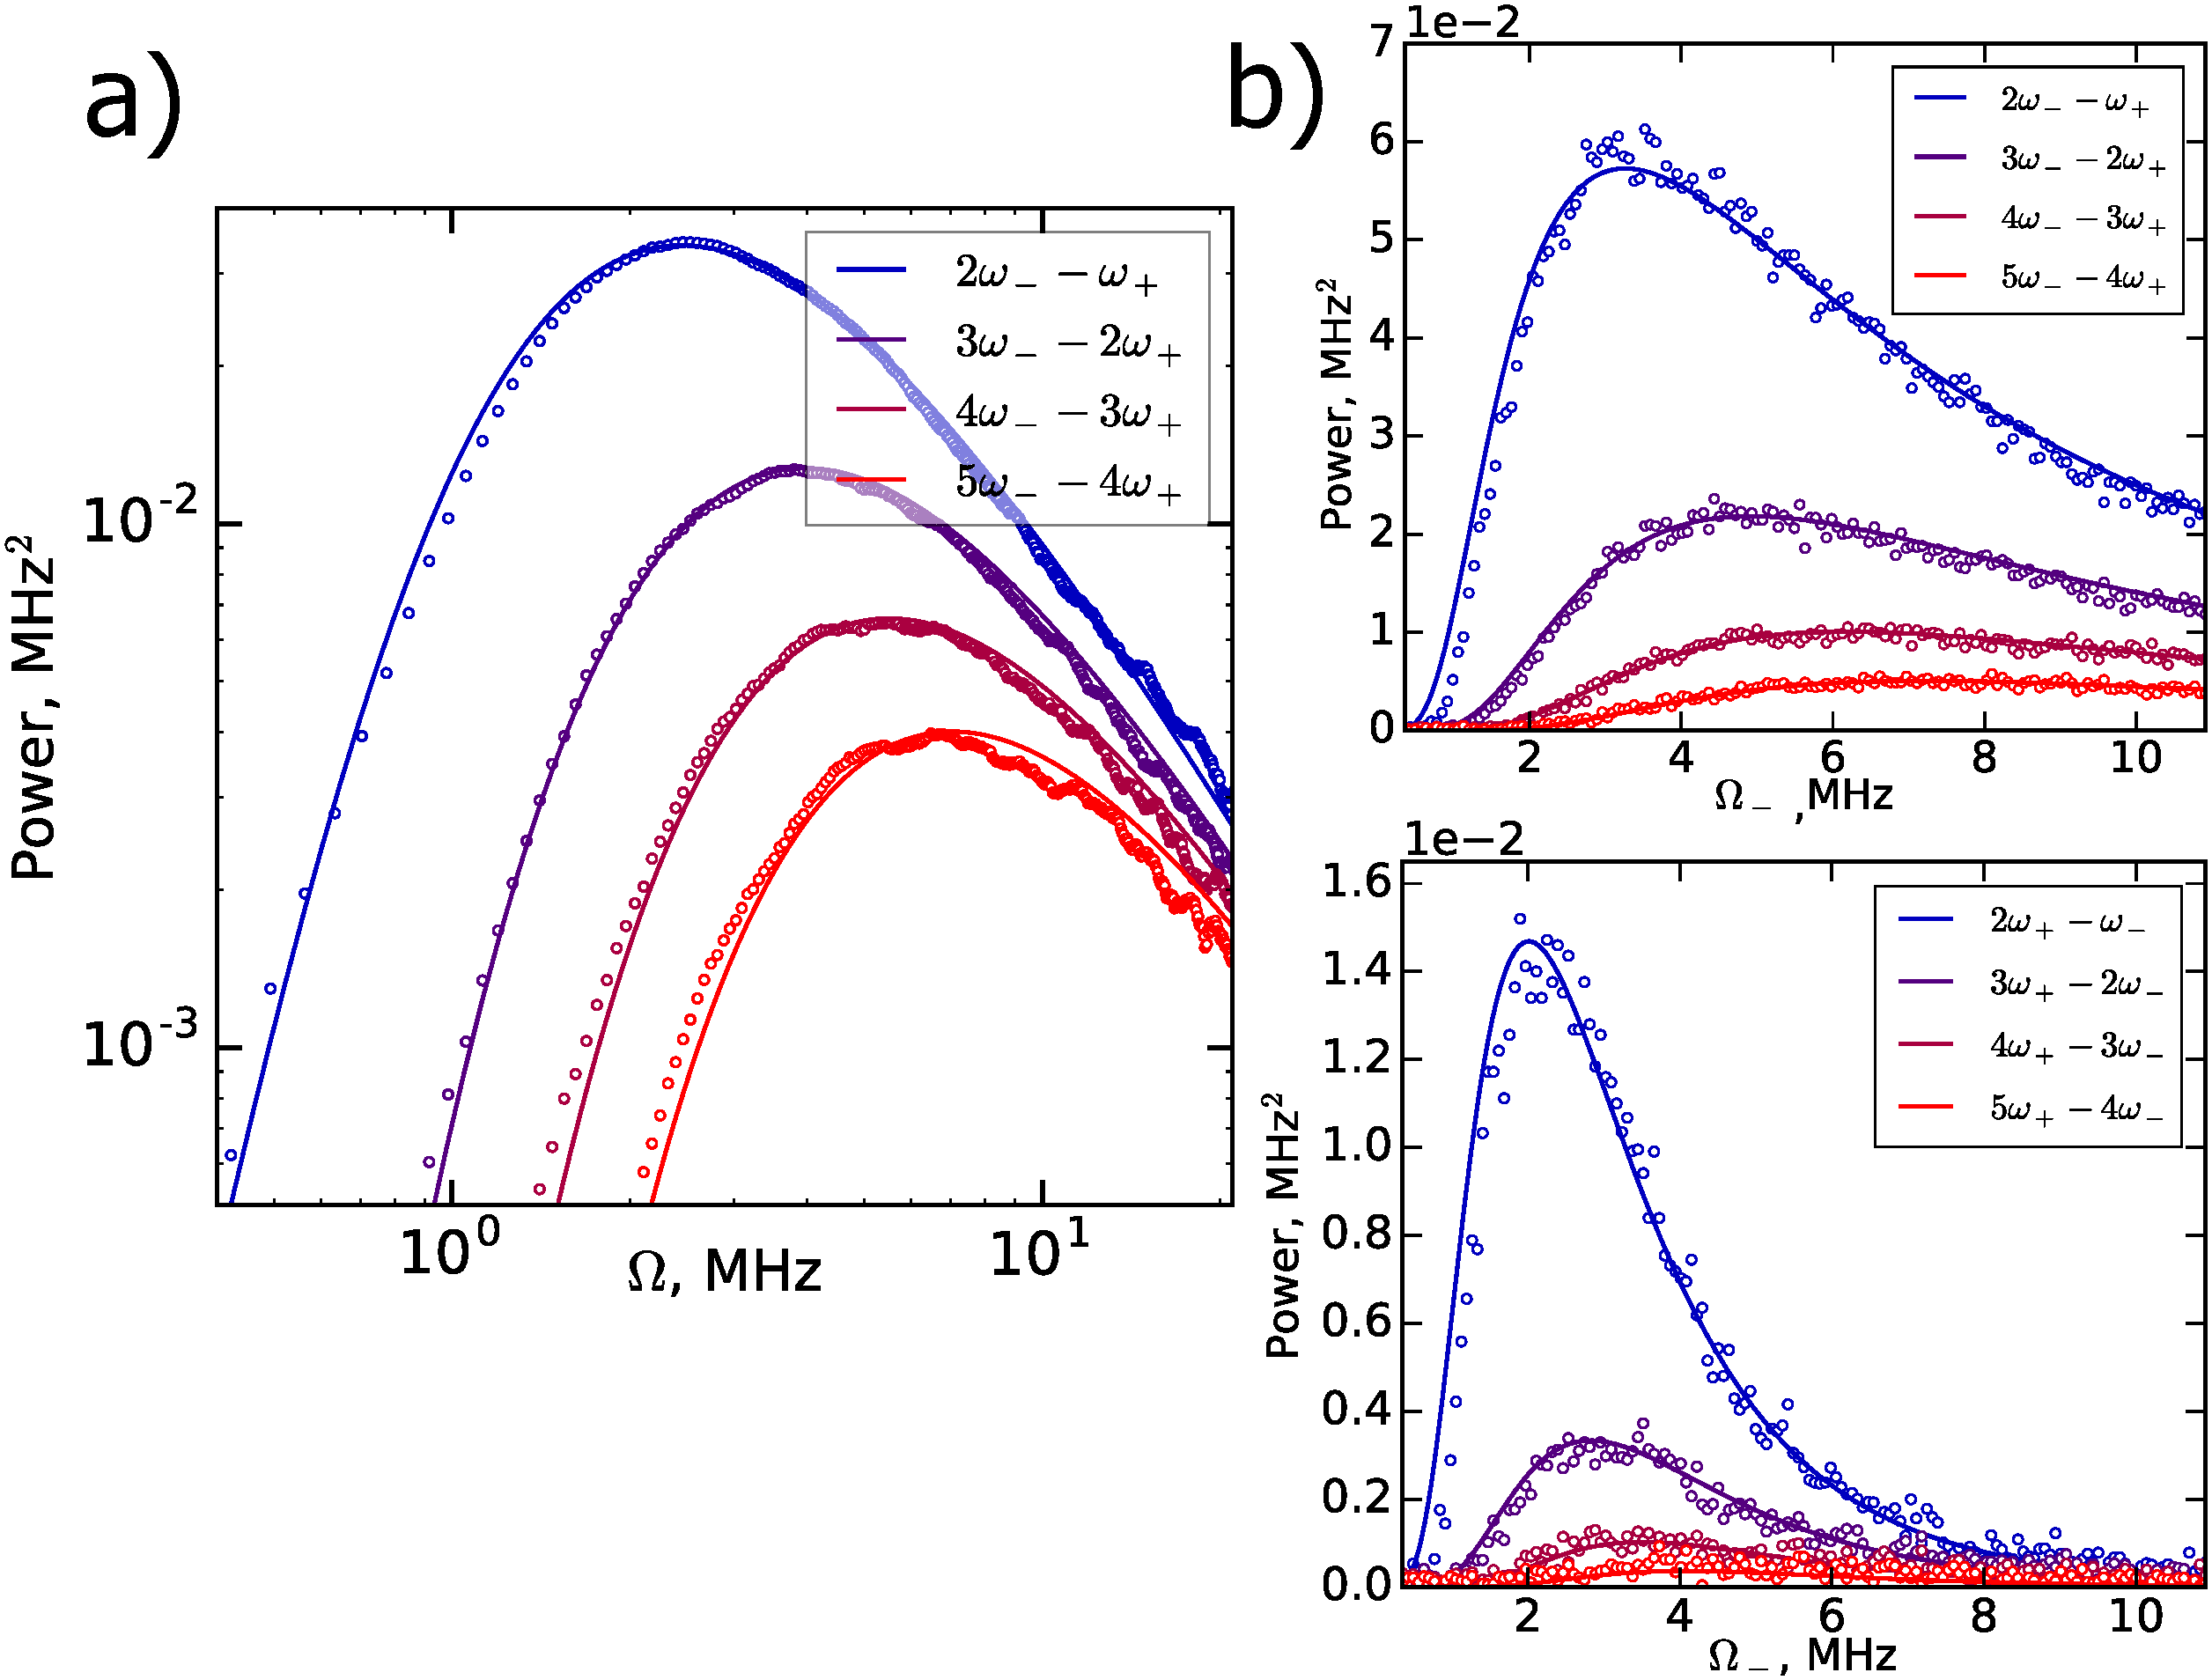
\includegraphics[width=0.7\textwidth]{ch_3/CWM_3-2_2.pdf}
	\caption{ Боковые спектральные компоненты эластично рассеянного света. Экспериментальные данные получены в случае  $\delta\omega=5$~кГц, все аналитические кривые \eqref{eq: mix_an} (сплошные линии) построены для значений $\Gamma_1 = 2.20$~MHz, $\Gamma_2=1.10$~MHz, $\Delta\omega=0$, $p=1,2,3,4$. Панель \textbf{(a)} соответствует случаю $\Omega_+=\Omega_- =\Omega$. \textbf{(b)} соответствует случаю, когда $\Omega_-$~на 1 дБ превосходит~$\Omega_+ $. Положительно смещенные компоненты (верхняя панель) в среднем в несколько раз меньше, чем отрицательно смещенные (нижняя панель). Это иллюстрирует высокую чувствительность компонент смешивания к дисбалансу возбуждающих сигналов.}
	\label{fig: fwm_fits}
\end{figure}

\textbf{Раздел 3.5} представляет результаты численного решения уравнений Блоха для кубита под действием бихроматической накачки. При этом боковые компоненты смешения появляются как Фурье-компоненты от численно рассчитанной зависимости временной динамики кубита. Полученные расчеты хорошо согласуются с аналитическими результатами в области применимости последних, но могут описывать и более сложные случаи, например, $\delta\omega\ge \Gamma_1$.

В \textbf{разделе 3.6} излагаются результаты волнового смешения при больших амплитудах накачки и ненулевых отстройках средней частоты: $\Delta\omega \ne 0$. В результате экспериментально наблюдаются расщепления в зависимости амплитуды боковых компонент от $\Delta\omega$ и $\Omega$, напоминающие расщепление Аутлера-Таунса для трехуровневой системы. Интересно отметить, что величина расщепления зависит от порядка компоненты, и определяется соотношением: $\Delta\omega=4\Omega/(2p+1)$.

\textbf{Раздел 3.7} посвящен обсуждению показанного эффекта квантового смешивания волн. Фактически, наблюдение спектров рассеянного сигнала визуализирует фотонную статистику состояния света, участвующего в смешивании. Те же результаты должны наблюдаться не только в случае приготовления нужного состояния в кубите, но и при распространении квантовых состояний в линии. Это открывает широкие перспективы по использованию кубита в линии в качестве сенсора, определяющего фотонную статистику. Поскольку измеряется только когерентно рассеянная часть света, данный подход работает только для состояний, обладающих когерентностью, однако даже при этом ограничении может быть весьма интересен для приложений квантовой электроники на чипе.

В \underline{\textbf{Главе 4}} изучается квантовое смешивание волн. Под этим названием понимается совокупность  физических эффектов, возникающих из-за квантовых свойств смешиваемого света, взаимодействующего посредством кубита в линии. 

\textbf{Раздел 4.1} описывает картину смешивания волн в случае, когда вместо непрерывных сигналов на кубит подаются непрерывные периодические последовательности коротких импульсов с длительностями $\Delta t \ll \Gamma_2$, см. Рис \ref{fig: bessel}, на тех же частотах $\omega_+, \omega_-$, что и в непрерывном случае. С точки зрения квантовых состояний света, разница практически отсутствует: статистика фотонов в коротком импульсе света также пуассоновская и описывается когерентным состоянием $\ket{\alpha}$. Можно говорить о том, что короткие импульсы имеют большую неопределенность по частоте, однако если последовательность достаточно большая и формируется из непрерывной волны, сохраняющей фазу, то частоты определены сколь угодно точно. Таким образом, общая характеристика спектра рассеянного сигнала --- наличие боковых компонент, возникающих из-за процессов смешивания волн --- справедлива и в импульсном случае. Однако, как известно, при взаимодействии с короткими импульсами кубит испытывает осциляции заселенности (Раби-осцилляции), и за счет сильной связи, эти осцилляции легко наблюдаются и в зависимости амплитуды рассеянного когерентного излучения от длительности импульса, см., например, \cite{abdumalikov2011dynamics}.
\begin{figure}[htb]\center
	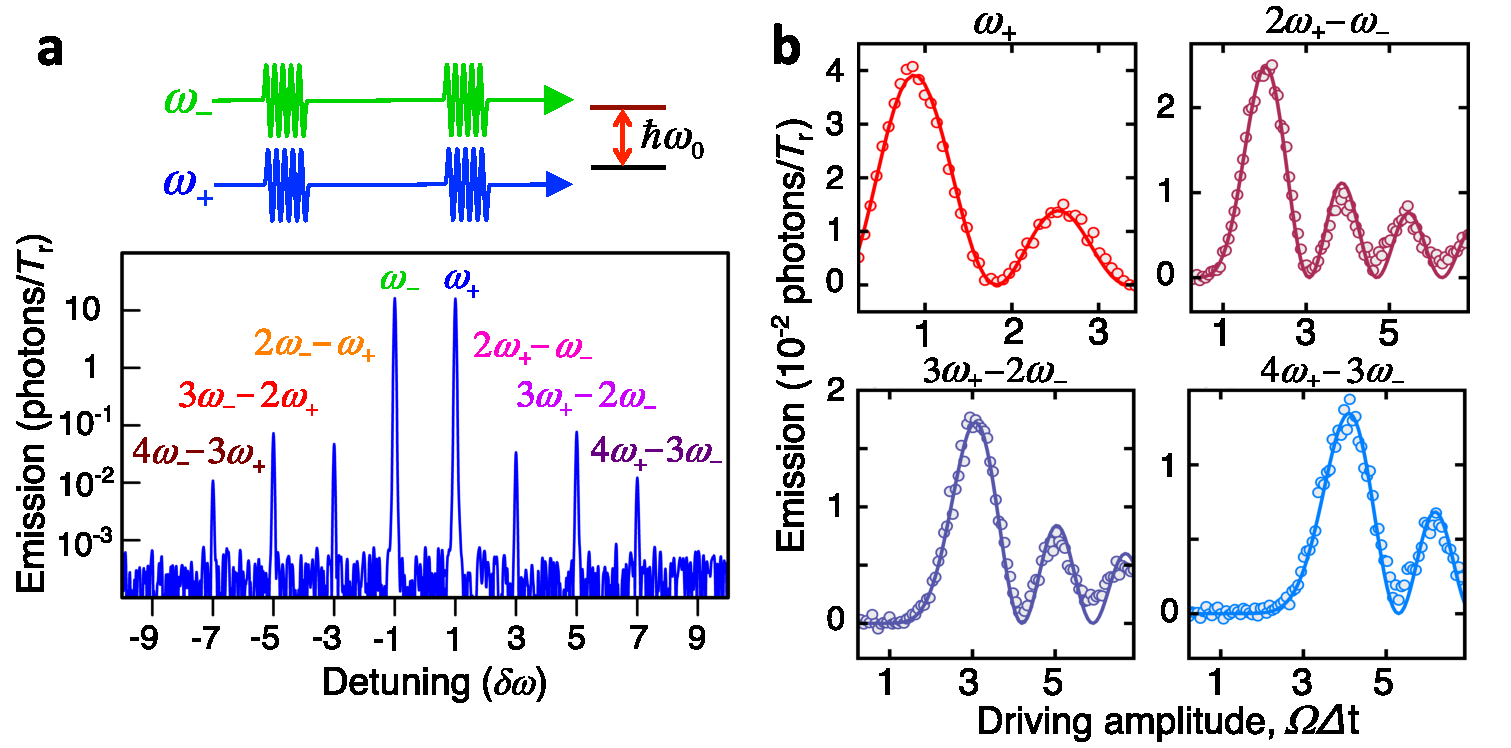
\includegraphics[width=0.7\textwidth]{ch_3/Fig2_rev3.pdf}	
	\caption{Смешивание последовательностей микроволновых импульсов  \textbf{(a)} Паттерн импульсов и спектр рассеянного сигнала, отчетливо видны боковые компоненты. \textbf{(b)} Зависимость интенсивности компонент от амплитуды накачки: точки соответствуют экспериментальным данным, линии --- расчетные значения согласно \eqref{eq:s_2k+1}}
	\label{fig: bessel}
\end{figure}
Поэтому можно ожидать похожих осцилляций и в боковых спектральных компонентах. Эти осцилляции наблюдались экспериментально, см. Рис. \ref{fig: bessel}. Рассматривая динамику двухуровневой системы под воздействием двух классических сигналов амплитуды $\Omega$, для среднего значения оператора эмиссии можно получить следующее выражение: 
\begin{equation}
\langle s^+_{2k+1}\rangle = \frac{(-1)^k}{2}J_{2k+1}(2\Omega t)e^{-(2k+1)\delta\omega t}, 
\label{eq:s_2k+1}
\end{equation}
где $J_{2k+1}$ --- функция Бесселя первого рода. Эта формула хорошо согласуется с экспериментальными зависимостями боковых пиков от величины $\Omega\Delta t$. Далее показано, что этот же ответ можно получить в представлении вторичного квантования и обобщить результаты для квантовых состояний поля. Концепция операторного подхода, применяемого в данной работе, проиллюстрирована на Рис. \ref{fig: opers}
\begin{figure}[htb]\center
	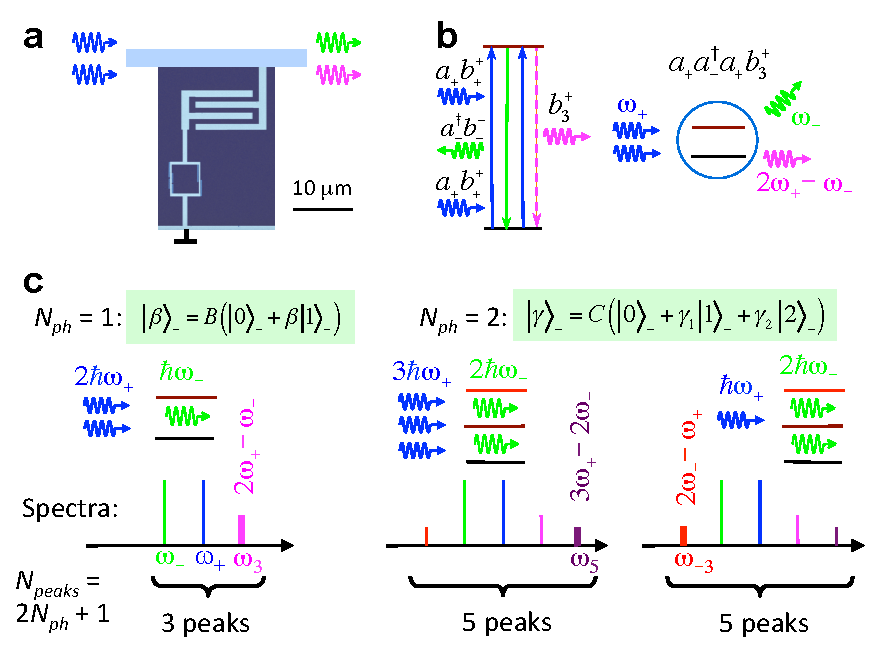
\includegraphics[width=0.7\textwidth]{ch_3/Fig1_NtC.pdf}
	\caption{К описанию процесса смешивания волн на кубите. \textbf{(a)} Схематичное изображение кубита и подаваемых микроволновых импульсов. \textbf{(b)} Схема переходов кубита под воздействием внешнего излучения и произведение операторов падающего $a$ и рассеянного $b$ сигнала. \textbf{(c)} Возможные четырех- и шестифотонные процессы, ответственные за появление боковых пиков на частотах $\omega_3$, $\omega_{-3}$ и $\omega_5$. }
	\label{fig: opers}	
\end{figure}
Во вращающейся с частотой $\omega_d$ системе отсчета введены операторы уничтожения/рождения фотона во внешнем поле на частотах $\omega_{\pm}$, обозначенные как $a_{\pm}=ae^{\pm i\delta\omega t}, a^{\dag}_{\pm} = a^{\dag}e^{\mp i\delta\omega t}$. Также вводятся операторы $b^-_{\pm}=\sigma_-e^{\pm i\delta\omega t}$~и~$b^+_{\pm}=\sigma_+ e^{\mp i\delta\omega t}$, рождающие/уничтожающие фотон на частотах $\omega_{\pm}$ за счет возбуждения/релаксации атома: возбуждаясь, атом обязательно испустит фотон через среднее время $\Omega$ из-за сильной связи с линией. Гамильтониан взаимодействия, таким образом, фактически представляет из себя гамильтониан Джейнса-Каммингса для двух мод поля, который  может быть записан в следующем виде:
\begin{equation}
H_t = i \hbar g\big(b_-^+ a_{-}  - b_-^-a^\dag_{-} + b_+^+ a_{+} - b^-_+ a^\dag_{+} \big).
\label{Hmb}
\end{equation}
Эта формула показывает, что возможны процессы как с поглощением, так и с испусканием фотонов на каждой из частот $\omega_{\pm}$. Однако, поскольку операторы содержат медленно меняющийся фазовый множитель $e^{\pm\delta\omega t}$, излучение будет наблюдаться и на смещенных частотах $\omega_{\pm(2k+1)} = (k+1)\omega_{\pm} - k\omega_{\mp}$. Записывая эволюцию системы $U = \exp(-\frac{i}{\hbar}H_t t)$, имеем:
\begin{equation}
\begin{split}
U =1 + \eta (b^-_m a^\dag_m - b^+_m a_m)  - \frac{\eta^2}{2!}(b^+_m b^-_j a_m a^\dag_j + b^-_m b^+_j a_m^{\dag} a_j)
- \\ - \frac{\eta^3}{3!} (b^-_{m-j+p} a^\dag_m a_j a^\dag_p - b^+_{m-j+p} a_m a_j^{\dag} a_p) +...,
\end{split}
\label{eq:ut2}
\end{equation}
нижние индексы принимают значения $\pm 1$. Мы используем соотношения $b^+_m b^-_j b^+_p = b^+_{m-j+p}$ потому что $b$-операторы должны удовлетворять таким же соотношениям, как и $s$-операторы: $s_m^+ s_j^- s_p^+ = e^{-i m\delta\omega t}\sigma^+ e^{i j\delta\omega t}\sigma^- e^{-i p\delta\omega t}\sigma^+ = e^{-i (m-j+p)\delta\omega t}\sigma^+ = s_{m-j+p}^+$. Определения $s$-операторов здесь расширены на произвольную $l$-моду как $s_l^\pm = e^{\mp i l\delta\omega t} \sigma^\pm$.  Это означает, например, что члены третьего порядка $a_+ a^\dag_- a_+ b^+_3$ и $a_- a^\dag_+ a_- b^+_{-3}$ создают однофотонное поле на частоте $\omega_{ge} \pm 3\delta\omega$. Член нижнего порядка в уравнении~\eqref{eq:ut2}, создающий однофотонное поле на частоте $\omega_{ge} \pm l\delta\omega$, где $l=2k+1$, состоит из $2k+2$ операторов: $2k+1$ $a$-операторов $a_\pm a^\dag_\mp a_\pm ... = (a_\pm a^\dag_\mp)^k a_\pm$ и один оператор $b_{\pm (2k+1)}^+$. Аккуратно подсчитывая вклад различных членов \cite{vakbib1}, можем получить выражение для оператора эволюции из начального состояния системы $\Psi = \ket{g, \alpha, \alpha}$ от момента $t$ до момента $t'$:
\begin{equation}
\begin{split}
U(t',t)\Psi(t) \approx \sum_{k=-\infty}^{\infty} \bigg[\frac{(-1)^k}{\alpha^{2k}}J_{2k}(\theta)\hat{A}_{2k}^{+-} |0\rangle_{2k} \otimes|\alpha,\alpha\rangle + \\
+ \frac{(-1)^k}{\alpha^{2k+1}}J_{2k+1}(\theta)\hat{A}_{2k+1}^{-} |1\rangle_{2k+1} \otimes|\alpha,\alpha\rangle \bigg], 
\end{split}
\end{equation}
где $\theta = 2\alpha g \Delta t$. Используя его, можно вычислить среднее значение от оператора $b^+_{2k+1} = |1\rangle_{2(k+p)+1}\langle 0|_{2p}$, где нижний индекс обозначает фазу и, соответственно, частоту излучения (см. выше
). Полагая $\alpha\gg1$ и выполняя ряд упрощений, получаем:
\begin{equation}
\langle b^+_{2k+1}\rangle = \frac{(-1)^k}{2} J_{2k+1}(2\Omega \Delta t),  
\label{eq:b2k1}
\end{equation}\

что совпадает с выражением \eqref{eq:s_2k+1}. В следующих разделах будет показано, что в рамках этого подхода можно описать также нетривиальный случай, когда импульсы посылаются с задержкой (без перекрытия), и происходит приготовление однофотонного состояния в кубите первым импульсом, и затем его смешивание со вторым импульсом. 

В~\textbf{Разделе 4.2} рассматривается квантовое смешивание волн в случае неперекрывающихся импульсов. По сравнению с представленным в предыдущем разделе экспериментом, мы меняем последовательность импульсов, разделяя их во времени, см. Рис. \ref{fig: qwm}.
\begin{figure}[htb]\center
	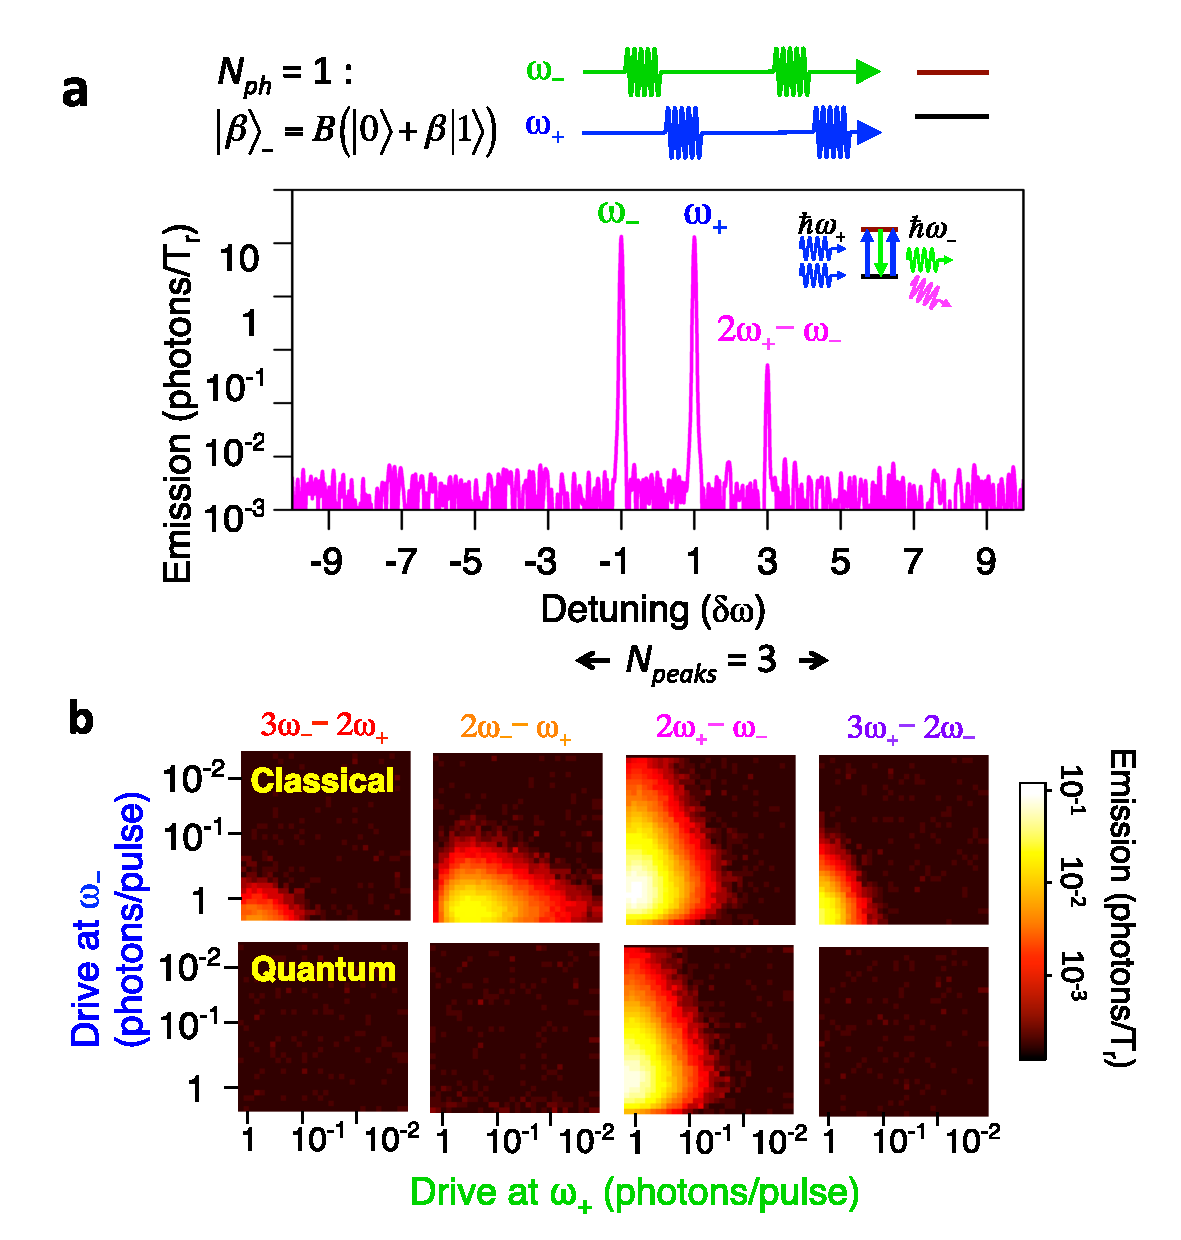
\includegraphics[width=0.7\textwidth]{ch_3/Fig3_NtC_rev_2.pdf}
	\caption{Квантовое смешивание волн. \textbf{(a)} Входной сигнал: импульсы на частоте $\omega_{-}$ опережают импульсы на частоте $\omega_+$, перекрытие между ними отвутствует. Помимо частот входных сигналов, в спектре остается лишь пик на частоте $\omega_{+3}=2\omega_+-\omega_-$, поскольку число фотонов частоты $\omega_-$ строго ограничено одним фотоном. \textbf{(b)} Сравнение интенсивностей в случае смешивания на Рис.  и квантового смешивания}
	\label{fig: qwm}	
\end{figure}
Можно сказать, что это нарушает симметрию обращения времени в возбуждающем поле, и соответственно, спектр рассеянного света становится несимметричным. Рис. \ref{fig: qwm} демонстрирует спектр, наблюдаемый в случае, когда импульс на частоте $\omega_+$ следует после импульса $\omega_-$. Спектр содержит единственный боковой пик на частоте $2\omega_+-\omega_-$ и в нем отсуствуют какие-либо другие компоненты, возникавшие ранее за счет смешивания волн. Обращение последовательности импульсов обращает спектр относительно центральной частоты $\omega_d$ (не показано). Качественное объяснение данного феномена состоит в следующем: первый импульс приводит кубит в состояние суперпозиции и, фактически, создает состояние света $\ket{\beta}_- = \frac{1}{\sqrt{1+\beta^2}}(\ket{0}_-+\beta\ket{1}_-)$ на частоте $\omega_-$, в котором имеется не больше одного фотона. Поэтому из всех нелинейных процессов становится возможным только один, в котором рождается фотон на частоте $2\omega_+-\omega_-$, испускается фотон на частоте $\omega_-$ и поглощается 2 фотона на частоте $\omega_+$. Чтобы подтвердить, что другие компоненты полностью отсутствуют, мы меняем амплитуды двух начальных сигналов в широких пределах и измеряем спектральную мощность излучения на частотах $\omega_{\pm3}$~и~$ \omega_{\pm5}$ для случая смешивания одновременных импульсов и смешивания с задержкой, см. Рис. \ref{fig: qwm}b). Результат показывает, что интенсивность на частоте $\omega_{+3}$ практически одинакова в обоих случаях, но в случае смешивания двух классических состояний возникает излучение и на других частотах, тогда как при наличии задержки и формирования неклассического состояния света другие процессы невозможны: излучение отсутствует во всем диапазоне изменения амплитуд накачки. Это подтверждает природу наблюдаемого эффекта. 
В \textbf{разделе 4.3} представлены результаты смешения двух неперекрывающихся последовательностей импульсов на трехуровневой системе. Еще одно подтверждение можно получить, рассеивая свет не на двухуровневой, а на трехуровневой системе. Как сказано выше, в качестве искусственного атома выступал потоковый кубит, спектр которого можно перестраивать внешним полем. Как видно из Рис. \ref{fig: spectra_3ls}, можно найти точку, в которой первые три уровня кубита эквидистантны, и изучать смешивание на трехуровневой системе. Нужно отметить, что нелинейность второго порядка по амплитуде поля у кубита отсутствует, поэтому двухфотонных процессов не происходит, и для классических состояний четырех-, шести-, восьмиволновое смешивание носит примерно такой же характер, как и в случае двухуровневой системы. Однако, существенно <<квантовый случай>> смешивания при наличии задержки между импульсами теперь дает другой спектр: в трехуровневой системе, когерентный импульс $\ket{\alpha}$ в общем случае оставляет кубит в состоянии $\ket{\gamma} = (\ket{0}+\gamma_1\ket{1}+\gamma_2\ket{2})/\sqrt{1+\gamma_1^2+\gamma_2^2}$, и поэтому появляется возможность наблюдать еще два процесса: один четырехфотонный c испусканием двух фотонов на частоте $\omega_-$ и один шестифотонный, c поглощением двух фотонов на частоте $\omega_-$ см. Рис. \ref{fig: qwm_3ls}. 
\begin{figure}[htb]\center
	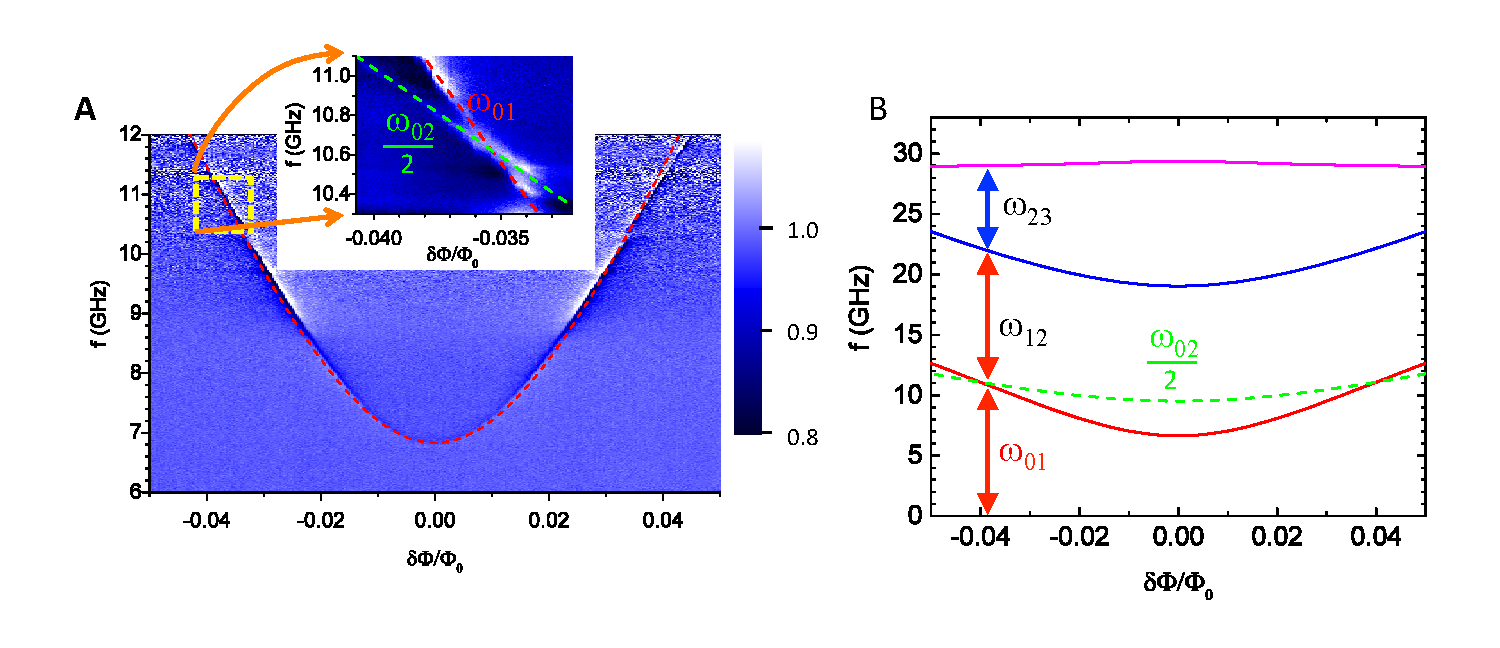
\includegraphics[width=1\textwidth]{ch_3/SFig2.pdf}
	\caption{Спектр потокового кубита. \textbf{(A)} Экспериментально измеренный спектр основного перехода потокового кубита. На вставке показано пересечение линий переходов 0-1 и 1-2.  \textbf{(B)} Численно рассчитанные энергии переходов}
	\label{fig: spectra_3ls}	
\end{figure}

\begin{figure}[htb]\center
	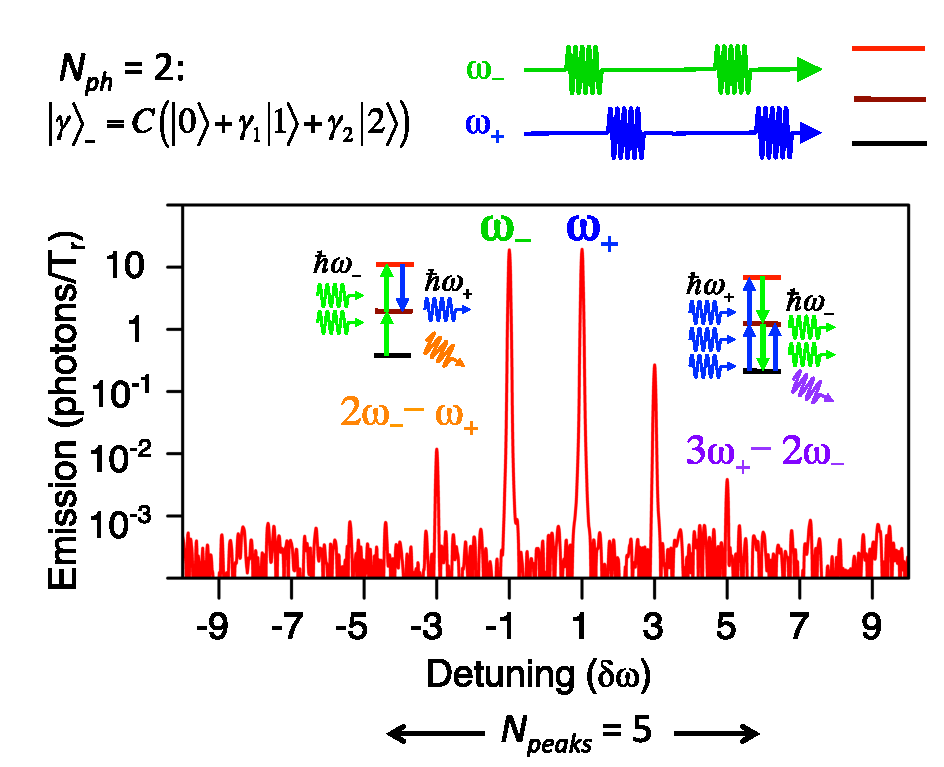
\includegraphics[width=0.6\textwidth]{ch_3/Fig4_NtC_rev2.pdf}
	\caption{Квантовое смешивание на трехуровневой системе.}
	\label{fig: qwm_3ls}	
\end{figure}
\textbf{Раздел 4.4}~посвящен аналитическому расчету зависимостей боковых компонент смешения от эффективной длительности импульсов (углов поворота $\theta_+$ и $\theta_-$). Получены формулы, описывающие зависимость каждой компоненты $\braket{\sigma^-_{2p+1}}$ атома от углов поворота, как для двухуровневого, так и для трехуровневого случая. Экспериментальная проверка этих результатов выходит за рамки диссертационной работы. 

\textbf{Раздел 4.5} представляет результаты численного расчета импульсной динамики системы. В частности, численный расчет дает качественно верные результаты в случае синхронных последовательностей импульсов, длительность которых сравнима с временем жизни кубита. 
\begin{figure}[htb]\center
	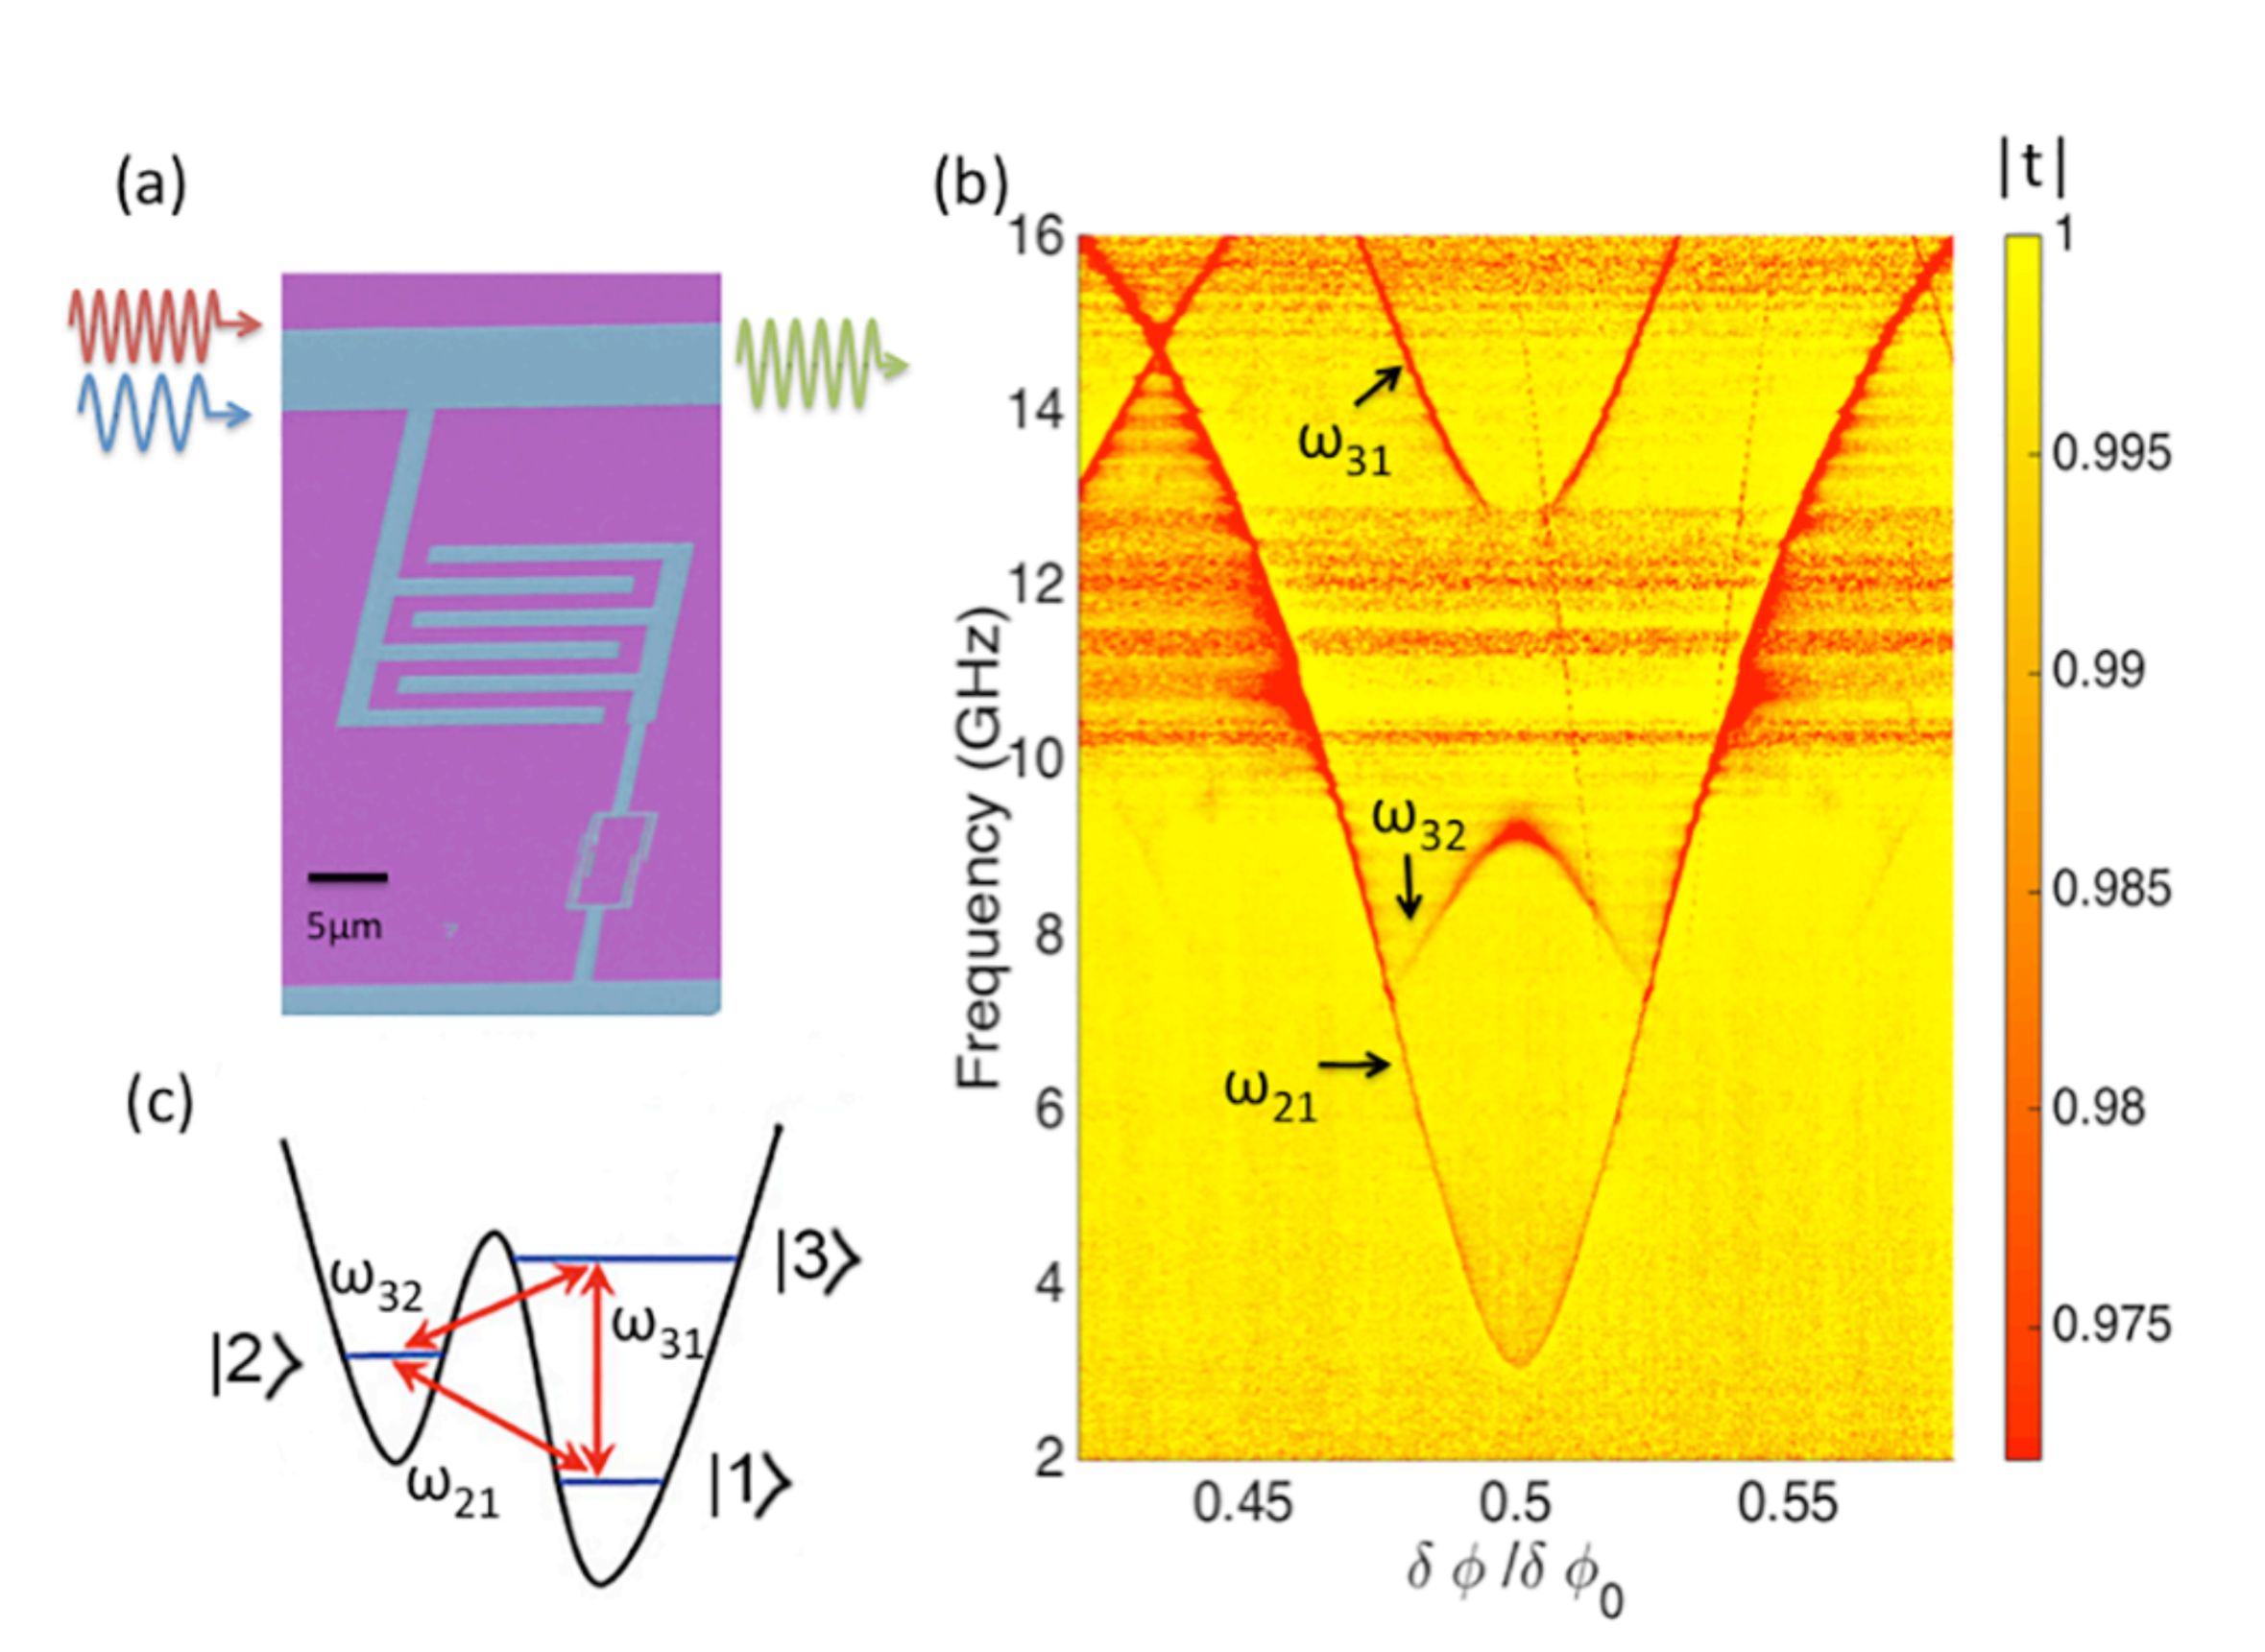
\includegraphics[width=0.7\textwidth]{ch_5/3wm_qubit.pdf}
	\caption{Потоковый кубит в качестве $\Delta$-системы. При отстройки от точки~$\delta\phi/\delta\phi_0=0.5$ все три перехода разрешены в дипольном приближении. }
	\label{fig: 3wm_qubit}	
\end{figure}

\textbf{\underline{Глава 5}} описывает эксперименты по наблюдению трехволнового смешивания на циклической $\Delta$-системе, практически не имеющей аналогов среди естественных физических систем (за исключением киральных молекул сложных газов \cite{Chiral}, оперировать с которыми достаточно неудобно, и кроме того, они неперестраиваемы по частоте). В отличие от устройств, подобных джозефсоновским параметрическим усилителям, которые демонстрируют трехволновое смешивание на основе классической нелинейности джозефсоновских переходов, здесь реализован другой способ с использованием трехуровневого искусственного атома с циклической конфигурацией уровней --- то есть, для каждой пары уровней дипольный излучательный переход разрешен. 

\textbf{Раздел 5.1} описывает кубит, выступающий в качестве циклической системы. Схема кубита и результаты измерения его спектров представлены на Рис. \ref{fig: 3wm_qubit}. Параметры усройства таковы, что три нижние частоты перехода попадают в доступный для измерений диапазон: $\omega_{21}/2\pi = 6.48$~ГГц, $\omega_{32}/2\pi = 8.35$~ГГц и $\omega_{31}/2\pi = 14.83$~ГГц, как схематично показано на Рис. \ref{fig: 3wm_qubit}c). 

\textbf{Раздел 5.2} описывает экспериментальные результаты трехволнового смешивания. Полученные зависимости интенсивностей излучения представлены на Рис. \ref{fig: 3wm_theor} и достаточно хорошо совпадают с расчетными для параметров $\Gamma_{21}/2\pi = 8 \text{ МГц}, \gamma_{21}/2\pi = 8 \text{ МГц}, \Gamma_{32}/2\pi = 38 \text{ МГц}, \gamma_{32}/2\pi = 42 \text{ МГц}, \Gamma_{31}/2\pi = 41 \text{ МГц}, \gamma_{31}/2\pi = 39.5 \text{ МГц} $. Таким образом, показан новый метод генерации когерентных микроволн при помощи трехволнового смешивания на трехуровневом искусственном атоме.

\textbf{Раздел 5.3} теоретически описывает процесс трехволнового смешивания. В приближении вращающейся волны, трехуровневый атом под действием двух возбуждающих сигналов, например, $\omega^d_{31}, \omega^d_{32} $, связывающих атомные состояния посредством дипольного взаимодействия $\hbar\Omega = d_{ij}V_{ij}$ может быть описан следующим гамильтонианом:
\begin{figure}[htb]\center
	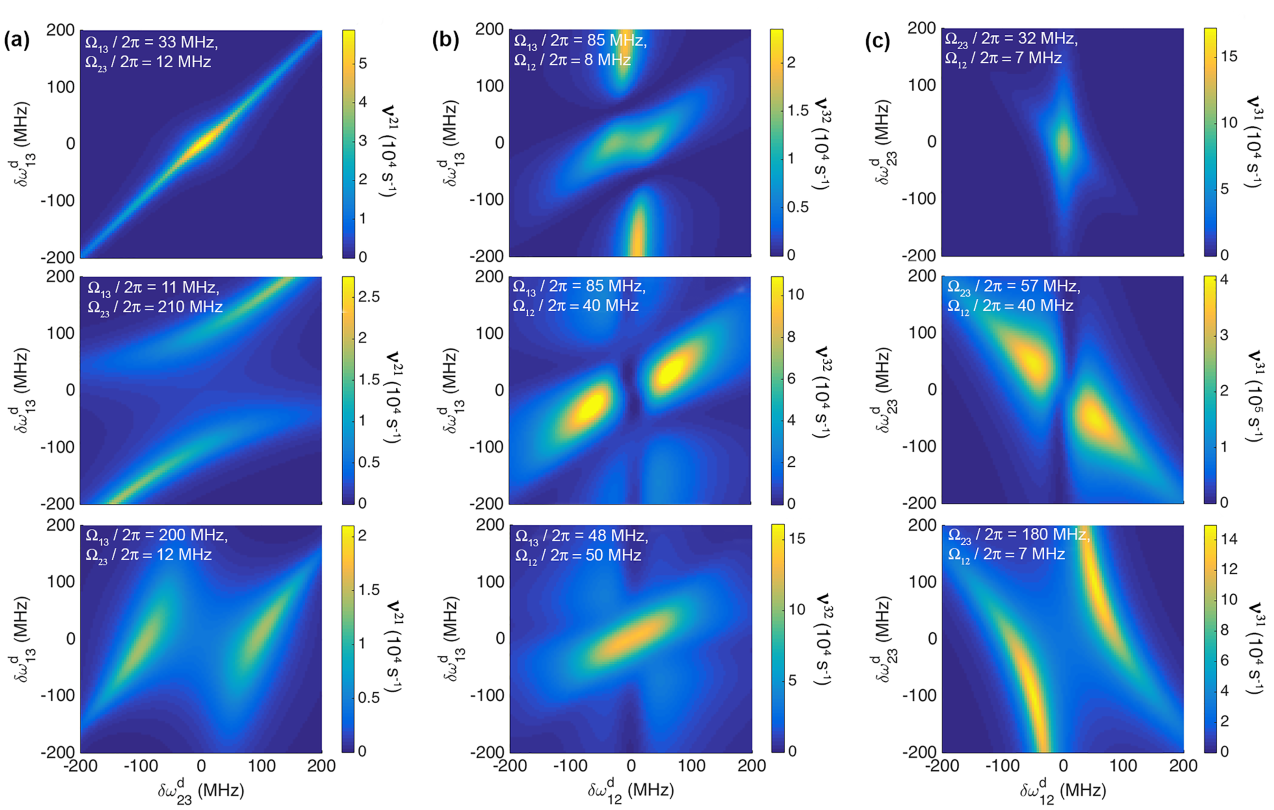
\includegraphics[width=0.9\textwidth]{ch_5/3wm_theor.png}
	\caption{Рассчитанные зависимости компонент трехволнового смешения в зависимости от амплитуд драйва и частотной отстройки.}
	\label{fig: 3wm_theor}	
\end{figure}
\begin{equation}
\begin{split}
H = & -\hbar (\delta\omega_{31}\sigma_{11} + \delta\omega_{23}\sigma_{22}) \\
    & -\hbar\Big[\frac{\Omega_{13}}{2}(\sigma_{13}+\sigma_{31})+\frac{\Omega_{23}}{2}(\sigma_{32}+\sigma_{23})\Big],
\end{split}
\end{equation}
где $\sigma_{ij} = \ket{i}\bra{j}$ --- оператор перехода. Гамильтонианы аналогичного вида получаются и в случае сигналов на частотах переходов 3-1 и 1-2, а также 1-2 и 2-3. Динамику системы можно описать с учетом процессов релаксации и дефазировки при помощи основного квантового уравнения с Линдбладовским членом:
\begin{equation}
\begin{split}
\hat{L}[\rho] = & \big(\Gamma_{31}\rho_{33} + \Gamma_{21}\rho_{22}\big)\sigma_{11} 
+ \big(\Gamma_{32}\rho_{33} - \Gamma_{21}\rho_{22}\big)\sigma_{22} \\
- &\big(\Gamma_{31}\rho_{33} + \Gamma_{23}\rho_{22}\big)\sigma_{33} 
- \sum_{i\ne j}\gamma_{ij}\rho_{ij}\sigma_{ij}
\end{split}
\end{equation}

\begin{figure}[h]\center
	\includegraphics[width=0.9\textwidth]{ch_5/3wm_exp.png}
	\caption{Экспериментально измеренные зависимости компонент трехволнового смешения в зависимости от амплитуд драйва и частотной отстройки. }
	\label{fig: 3wm_exp}	
\end{figure}
Находя стационарное решение основного уравнения ($\dot{\rho}=0$), можно вычислить среднее от оператора $\langle\sigma_{ij}\rangle=\text{Tr}(\sigma_{ij}\rho)=\rho_{ij}$. Напряжение на частоте эмиссии можно найти как $V_{ij}^{em} = \hbar\Gamma_{ij}/d_{ij}^2 \cdot \langle\sigma_{ij}\rangle$, и для мощности когерентного излучения на частоте $\omega$ в единицах потока фотонов получаем следующее выражение:

\begin{equation}
\nu^{ij}=\frac{S_{ij}(\omega)}{\hbar\omega} = \frac{\Gamma_{ij}}{2}\langle\sigma_{ij}(\omega)\rangle^2.
\end{equation}
Полученные для каждой возможной пары возбуждающих сигналов зависимости $\nu^{ik}$ от отстройки $\delta\omega_{ij}, \delta\omega_{jk}$ приведены на Рис. \ref{fig: 3wm_theor} для некоторых фиксированных значений амплитуд $\Omega_{ij}, \Omega_{jk}$. 

\underline{\textbf{Глава 6}} посвящена результатам измерений кубита, асимметрично связанного с двумя полупространствами, одно из которых может использоваться для контроля состояния, которое затем излучается в другое полупространство. 

\textbf{Раздел 6.1} описывает идею асимметрично связанного кубита и представляет оптический аналог данной схемы --- атом, расположенный позади малого отверстия в непрозрачном экране.

\textbf{Раздел 6.2} представляет дизайн и параметры кубита. \textbf{Раздел 6.3} описывает схему эксперимента. \textbf{Раздел 6.4} представляет результаты многоуровневой спектроскопии кубита, позволяющей восстановить положение трех нижних энергетических уровней. В \textbf{разделе 6.5} измеряется эффективность изучаемого кубита в качестве источника одиночных фотонов, показано, что она составляет примерно 70\%. Также в этом разделе представлены результаты измерений формы фотона, а также корреляционной функции первого порядка для состояний $\ket{1}$ и $(\ket{0}+\ket{1})/\sqrt{2}$, согласующиеся с ранее представляемыми другими научными группами данными похожих измерений. В \textbf{разделе 6.6} показано возникновение расщепления Аутлера-Таунса на трехуровневой подсистеме изучаемого потокового кубита. 
%Можно сослаться на свои работы в автореферате. Для этого в файле
%\verb!Synopsis/setup.tex! необходимо присвоить положительное значение
%счётчику \verb!\setcounter{usefootcite}{1}!. В таком случае ссылки на
%работы других авторов будут подстрочными.
%\ifnumgreater{\value{usefootcite}}{0}{
%Изложенные в третьей главе результаты опубликованы в~\cite{vakbib1, vakbib2}.
%}{}
%Использование подстрочных ссылок внутри таблиц может вызывать проблемы.
%
%В \underline{\textbf{Главе 4}} приведено описание 
%

В \underline{\textbf{Заключении}} приведены основные результаты работы, которые заключаются в следующем:
%% Согласно ГОСТ Р 7.0.11-2011:
%% 5.3.3 В заключении диссертации излагают итоги выполненного исследования, рекомендации, перспективы дальнейшей разработки темы.
%% 9.2.3 В заключении автореферата диссертации излагают итоги данного исследования, рекомендации и перспективы дальнейшей разработки темы.
\begin{enumerate}
  \item Спроектированы и изготовлены и исследованы образцы потоковых кубитов, сильно связанных с континумом электромагнитных мод как в геометрии боковой связи (кубит в линии), так и в геометрии прямой связи (кубит, асимметрично связанный с двумя полупространствами);
  \item Воспроизведены базовые квантовооптические эксперименты с одиночными кубитами --- в частности, измерена однотоновая спектроскопия в зависимости от внешнего магнитного поля, зависимость формы линии кубита от амплитуды накачки, измерен триплет Моллоу, приведены результаты различных импульсных измерений, в частности осцилляции Раби и свободное затухание Рамзи;
  \item Получен \textit{эффект непрерывного волнового смешения} на кубите в линии. Показано, что эластичная часть спектра излучения, образовывающегося при рассеянии на кубите двух непрерывных монохроматических волн, несущие частоты которых $\omega_+, \omega_-$ отличается от частоты кубита на $\delta\omega \ll \Gamma_1$, состоит из большого количества пиков аппаратной ширины на частотах $\omega_{\pm(2p+1)}= (p+1)\omega_{\pm}-p \omega_{\mp}$.  При этом возможность наблюдения пиков порядка $p$ ограничено только наличием шума усилителя, используемого в измерительном тракте;
  \item Получена формула, которая описывает амплитуду каждого из вышеупомянутых когерентных компонент (пиков) $\Omega^{sc}_{\pm(2p+1)}$ в зависимости от амплитуды волн накачки $\Omega_+, \Omega_-$ и остальных параметров кубита. Проверено, что экспериментально измеренные амплитуды соответствуют полученной формуле как в случае $\Omega_- = \Omega _+ = \Omega$, так и в случае $\Omega_+ \ne \Omega_-$, причем амплитуды боковых пиков исключительно чувствительны к неравентству амплитуд волн накачки;
  \item Показано, что отношение амплитуд двух соседних пиков, отвечающих отличающимся на единицу значениям $p$, не зависит от $p$, а определяется только параметрами системы. 
  \item Показан эффект, аналогичный расщеплению Аутлера-Таунса и наблюдающийся для боковых компонент при синхронном увеличении эффективной частоты Раби каждой из волн накачки. Показано, что величина расщепления зависит от порядка смешения и выражается соотношением $2\Delta\omega = 8\Omega/(2p+1)$.
  \item Приведены аргументы в пользу того, что эффект непрерывного волнового смешения может использоваться для определения фотонной статистики стационарного или квазистационарного поля в волноводе;
  \item Исследован эффект \textit{импульсного волнового смешения} на кубите в линии. Показано, что при рассеивании на кубите последовательности коротких импульсов длительностью $\Delta t \ll 1/\Gamma_1$ с несущими частотами $\omega_+, \omega_-$, определенными выше, попадающими на кубит одновременно (без задержки) с периодом $T_r \gg 1/\Gamma_1$ наблюдается бесселевская динамика в зависимостях $\Omega^{sc}_{\pm(2p+1)}(\Omega \Delta t)$, где $\Omega=\Omega_+=\Omega_-$ --- амплитуда волн накачки. Пренебрегая затуханием, получена точная формула \eqref{Bessel_power} для энергии в числе фотонов на время жизни кубита, излучаемой в каждой из боковых компонент, которая описывает экспериментальные результаты без подгоночных параметров. 
  \item Исследован эффект \textit{квантового волнового смешения} на кубите в линии. Показано, что если ввести достаточно большую задержку между импульсами с различными частотами (настолько большую, чтобы импульсы не перекрывались во времени), то спектр эластичного рассеяния модифицируется особенным образом: остается единственный боковой пик на частоте $\omega_{-3}$, если импульс на частоте $\omega_-$ следует за импульсом на частоте $\omega_+$, либо же пик на частоте $\omega_+$, если импульс $\omega_+$ следует за импульсом на частоте $\omega_-$. Предложено качественное объяснение наблюдаемому эффекту: кубит может <<запомнить>> только единственный квант возбуждения, другими словами --- поглотить единственный фотон из первого импульса, что запрещает все процессы многофотонного рассеяния, кроме единственного процесса на частоте $2\omega_--\omega_+$
  \item Получены аналитические выражения для зависимости амплитуды пиков на частотах $\omega_+, \omega_- \text{и} \omega_{+3}$ от эффективного угла поворота $\Omega\Delta t$.
  \item Исследован эффект квантового волнового смешения на \textit{трехуровневой эквидистантной квантовой системе}, которой является потоковый кубит при определенном значении внешнего магнитного потока. Показано, что при облучении неперекрывающимися импульсами возникают боковые пики на частотах $\omega_{+5}, \omega_{+3} \text{ и } \omega_{-3}$. Качественная интерпретация эффекта состоит в том, что трехуровневая система может находится в состоянии, где число возбуждений равно 2, и таким образом становятся разрешенными те процессы, где число фотонов из импульса на частоте $\omega_-$ не превышает 2.
  \item Построена модель трехуровневой эквидистантной системы, возбуждаемой классическим полем, в рамках этой модели получены аналитические зависимости амплитуд боковых компонент от эффективного угла поворота $R\Omega \Delta t$, где $R$ зависит от дипольного момента верхнего перехода системы. 
  \item Впервые экспериментально получено и исследовано трехволновое смешение на $\Delta-$системе в трех возможных режимах, когда осуществляется резонансная накачка двух переходов и изучается когерентно рассеянный сигнал на частоте третьего перехода. Показано, что экспериментальные результаты во всех режимах хорошо согласуются как с аналитическим решением основного квантового уравнения, описывающего динамику системы, так и с численным решением.  
  \item Проведено экспериментальное исследование потокового кубита, асимметрично связанного с двумя полупространствами. Показано, что двухтоновая спектроскопия позволяет увидеть рассеянное поле и восстановить спектр кубита до третьего возбужденного уровня включительно. Для конкретного образца проведена оценка эффективности генерации одиночных фотонов, которая составила 70\%. Также изучено расщепление Аутлера-Таунса на трехуровневой системе и показано, что максимум когерентного излучения наблюдается в случае, когда Раби-частота накачки совпадает с константой релаксации накачиваемого перехода.
\end{enumerate}


Автор выражает глубокую и искреннюю благодарность научному руководителю Астафьеву Олегу Владимировичу за внимание, доброе отношение и готовность участвовать в обсуждении результатов и помогать в решении текущих проблем. Также автор благодарит весь коллектив лаборатории искусственных квантовых систем МФТИ, а также коллектив лаборатории сверхпроводящих метаматериалов (МИСиС) и лаборатории сверхпроводимости (ИФТТ РАН). 
%%\newpage
%При использовании пакета \verb!biblatex! список публикаций автора по теме
%диссертации формируется в разделе <<\publications>>\ файла
%\verb!../common/characteristic.tex!  при помощи команды \verb!\nocite! 

\ifdefmacro{\microtypesetup}{\microtypesetup{protrusion=false}}{} % не рекомендуется применять пакет микротипографики к автоматически генерируемому списку литературы
\ifnumequal{\value{bibliosel}}{0}{% Встроенная реализация с загрузкой файла через движок bibtex8
  \renewcommand{\bibname}{\large \authorbibtitle}
  %\nocite{*}
 % \insertbiblioauthor           % Подключаем Bib-базы
  %\insertbiblioother   % !!! bibtex не умеет работать с несколькими библиографиями !!!
}{% Реализация пакетом biblatex через движок biber
  \ifnumgreater{\value{usefootcite}}{0}{
  %\nocite{*} % Невидимая цитата всех работ, позволит вывести все работы автора
%  \insertbiblioauthorcited      % Вывод процитированных в автореферате работ автора
  }{
  \insertbiblioauthor           % Вывод всех работ автора
  %\insertbiblioauthorgrouped    % Вывод всех работ автора, сгруппированных по источникам
  %\insertbiblioauthorimportant  % Вывод наиболее значимых работ автора (определяется в файле characteristic во второй section)
  \insertbiblioother            % Вывод списка литературы, на которую ссылались в тексте автореферата
  }
}
\ifdefmacro{\microtypesetup}{\microtypesetup{protrusion=true}}{}

